% Autor: Carles Marin (Claude, Anthropic, como asistente de investigacion IA).
% Parte V, edicion castellana de ghu_observability.tex. Lo que el potencial de Higgs no puede ver:
% materia del bulk que no puede ayudar a seleccionar una condicion de contorno. El potencial es un
% solo operador trazado dos veces: una dimension y un indice.
% NO es la afirmacion de un borrador anterior: "la mitad coset es lo unico que ve la conjugacion de
% carga". Eso es FALSO, retirado el 2026-07-30 y contradicho en letra impresa (GATE_KKKY.md).
% Esta edicion se hace cuando la inglesa deja de moverse, y traducir es una segunda revision.
% Compilar: pdflatex x2.  Cada numero se regenera desde ../*.py, con salida en ../outputs/.
\documentclass[11pt,a4paper]{article}
\usepackage[utf8]{inputenc}
\usepackage[T1]{fontenc}
\usepackage[spanish,es-noshorthands]{babel}
\addto\captionsspanish{\renewcommand{\tablename}{Tabla}}  % la casa dice Tabla, no Cuadro (Parte II)
\usepackage{amsmath,amssymb,amsthm}
\usepackage{booktabs}
\usepackage{longtable}   % el libro mayor tiene que romper por paginas, o deja una casi en blanco
\usepackage{dsfont}      % \mathds{1}: amssymb no tiene un 1 de pizarra y sustituye un glifo ajeno
\usepackage[table,dvipsnames]{xcolor}
\usepackage{graphicx}
\usepackage{tikz}
\usetikzlibrary{shapes.geometric,arrows.meta,positioning,fit,backgrounds,patterns,calc}
\usepackage{geometry}
\geometry{margin=2.4cm}
\usepackage[colorlinks=true,linkcolor=RoyalBlue,citecolor=BrickRed,urlcolor=RoyalBlue]{hyperref}
\usepackage{caption}
\captionsetup{font=small,labelfont=bf}
\newtheorem{theorem}{Teorema}
\newtheorem{lemma}{Lema}
\newtheorem{corollary}{Corolario}
\newtheorem{proposition}{Proposición}
\newtheorem{observation}{Observación}
\newcommand{\ZZ}{\mathbb{Z}}
% la matriz identidad: \mathbb{1} no tiene glifo en msbm y se imprime como \nVdash sin avisar
\newcommand{\one}{\mathds{1}}
\newcommand{\su}[1]{SU(#1)}
\newcommand{\Sig}{\Sigma_\lambda}
\newcommand{\Dl}{D_\lambda}

% el hilo: cada seccion cierra con la pregunta que abre la siguiente
\newcommand{\bridge}[1]{\par\medskip\noindent
  \textcolor{hdrblue!45}{\rule{2.2cm}{0.6pt}}\;\;\parbox[t]{0.84\textwidth}{\small\itshape
  \textcolor{hdrblue!85}{#1}}\par\medskip}

% un recuadro para las ecuaciones sobre las que se sostiene el paper, y solo esas
\newsavebox{\keyeqbox}
\newenvironment{keyeq}
  {\begin{center}\setlength{\fboxsep}{9pt}\setlength{\fboxrule}{0.8pt}%
   \begin{lrbox}{\keyeqbox}\begin{minipage}{0.88\textwidth}}
  {\end{minipage}\end{lrbox}%
   \fcolorbox{hdrblue!55}{hdrblue!6}{\usebox{\keyeqbox}}\end{center}}
\definecolor{okgreen}{RGB}{0,140,54}
\definecolor{hdrblue}{RGB}{31,78,121}
\definecolor{softgrey}{RGB}{238,242,247}
\definecolor{warmred}{RGB}{178,34,34}

\title{\textbf{\Large Lo que el potencial de Higgs no puede ver:\\[2pt]
materia del bulk que no puede ayudar a seleccionar una condición de contorno}\\[7pt]
\large\textnormal{\itshape La paridad del winding es la etiqueta de componente de $O(4)$, luego el
potencial es un solo operador trazado dos veces --- una \textnormal{dimensión} y un
\textnormal{índice}; el signo de contorno cabalga sólo sobre el índice, y queda ciego en una
clase que clasificamos y contamos en forma cerrada}\\[8pt]
\normalsize\textnormal{Parte V --- unificación gauge-Higgs $\su4$ en 6D: los coeficientes a un
bucle publicados por tres artículos distintos, reproducidos sólo desde teoría de
representaciones, y una regla de selección sobre el contenido de materia que no cuesta nada
aplicar}}
\author{Carles Mar\'in\thanks{Investigador independiente, \texttt{karlesmarin@gmail.com}.
Los cálculos se realizaron y contrastaron con Claude (Anthropic) como asistente de investigación
IA contra una verdad de referencia común verificable por máquina; cada número de este
artículo se regenera desde los guiones auxiliares, cuya salida se archiva junto a ellos.}}
\date{\today}

\begin{document}
\maketitle

\begin{abstract}
\noindent
Las Partes~I--IV de esta serie construyeron una pieza de teoría de representaciones y dejaron
implícito su propósito físico. Este artículo lo suministra. La propia matriz de traslación
de la Parte~III, $U_6=P_2P_0^{-1}$, tiene determinante $-1$, luego no está en la componente
identidad del grupo de estructura; la consecuencia es que la paridad del número de winding es la
etiqueta de componente de $O(4)$, y todo el potencial de línea de Wilson a un bucle del modelo es
\emph{dos especializaciones de Schur de una misma partición}, $\Sig(t)=s_\lambda(1,1,t,t^{-1})$ en
la componente identidad y $\Dl(t)=s_\lambda(1,-1,t,t^{-1})$ --- el objeto de la Parte~IV --- en el
coset de reflexión. La afirmación está anclada a números que no produjimos nosotros: la forma
estándar en que este campo escribe su potencial a un bucle, $\{A+B(-1)^{k_2}\}$, tiene coeficientes
que \emph{son} $(\Sig\pm\Dl)/2$, y los números publicados de tres artículos distintos --- en tres
grupos, dos dimensiones y dos orbifolds --- se reproducen desde teoría de representaciones sin
ajustar nada. El par es un solo objeto leído dos veces: con $\sigma$ la paridad del orbifold y
$g_t$ el elemento de línea de Wilson, $\sigma g_t$ es el alfabeto del coset, luego
$\Sig=\mathrm{Tr}(g_t)$ y $\Dl=\mathrm{Tr}(\sigma g_t)$ --- una traza y una traza torcida de un mismo
elemento sobre un mismo espacio, una dimensión y un índice. Lo que sigue es un enunciado sobre lo
que un potencial así puede y no puede ver. Cada multiplete de materia lleva un signo discreto de
condición de contorno --- en la notación que Haba, Hosotani y Kawamura usan desde 2004, el
producto $\eta=\eta_0\eta_1$ de los dos signos asociados a las paridades del orbifold --- y ese signo
multiplica el carácter del coset y nada más. De ahí:
$(\lambda,\eta)\sim(\lambda^*,\eta(-1)^{\lambda_1})$ es una identidad observacional --- demostrada, y
verificada sobre el rango barrido como la única colisión que hay --- y $\eta$
es inobservable \emph{exactamente} en $\mathcal Z$, la clase de anulación de la Parte~IV, cuya
clasificación en forma cerrada es por tanto una clasificación de los multipletes que no pueden
ayudar a seleccionar una condición de contorno. El puente con la literatura más antigua es exacto
y ensancha el enunciado: para cualquier representación, un par de paridades de orbifold ve un
multiplete a través de exactamente tres caracteres,
$N^{(\varepsilon_0,\varepsilon_1)}=\frac14[\dim+\varepsilon_0\chi(P_0)+\varepsilon_1\chi(P_1)
+\varepsilon_0\varepsilon_1\chi(P_0P_1)]$, y $\eta$ multiplica el último y sólo el último ---
de modo que el teorema no es una propiedad de un modelo hexadimensional sino de la clasificación
$[p;q,r;s]$ misma. Un corolario resuelve una diferencia de régimen con la que esperábamos tener
que convivir: como la forma cerrada de la Parte~IV tiene coeficientes de un solo signo, $\Dl(1)=0$ si
y sólo si $\Dl\equiv0$, luego el signo es invisible a fase de Wilson nula --- donde calcula la
literatura en 5D --- si y sólo si lo es a toda fase. Otros tres enunciados se demuestran o se miden
en vez de afirmarse: la clase ciega se cuenta en forma cerrada, $\lceil(k+1)^2/2\rceil$ en
$\lambda_1=2k+1$ y nunca para $\lambda_1$ par --- verificado por máquina en Lean~4, y encadenado al
certificado que la Parte~III ya tenía, de modo que el recuento es un teorema sobre el determinante
bialternante y no sobre un predicado elegido por ser contable; la asimetría entre las dos mitades se
remonta a que las letras congeladas sean un conjunto completo de raíces de la unidad, lo que pone
cada cero del carácter del coset sobre el círculo unidad y ninguno de los del carácter identidad, de
modo que la amplitud del coset se anula sólo en fases de Wilson \emph{racionales}; y el mismo test,
aplicado a las condiciones de contorno mismas, muestra que $\lfloor(N+1)^2/2\rfloor$ de las
$(N+1)^2$ clases de equivalencia admiten sector coset siquiera --- también verificado por máquina, y
para todo rango en vez de sobre un rango barrido, porque el par de bloques
$(\#\{P_0{=}{+}1\},\#\{P_1{=}{-}1\})$ resulta ser un invariante de clase completo ---, lo que parte
la cuestión de la invisibilidad en un caso geométrico y otro de teoría de representaciones, y sólo el
segundo es nuestro. Un paso más allá de un solo multiplete sale entonces gratis: si los multipletes
no ciegos de un contenido de materia comparten un mismo signo efectivo, el contenido es ciego sólo si
lo es cada multiplete suyo --- de modo que \emph{la ceguera colectiva exige frustración de signos}, y
la degeneración que queda para la continuación es la mitad frustrada. El alcance se enuncia y no se
entierra: todo aquí es sobre un \emph{modelo}, el teorema es \emph{por multiplete}, y todo lo que corre la maquinaria hacia adelante --- predecir un espectro en
vez de excluirlo --- se reserva deliberadamente para la Parte~VI. \emph{Retirado antes de publicar, y
registrado porque el registro vale tanto como el resultado:} un borrador anterior de
\S\ref{sec:obs} afirmaba que la mitad coset es lo único observable del modelo que ve la
conjugación de carga. No lo es; la conjugación de carga es aquí invisible sin condiciones, y
Kawamura, Kodaira, Kojima y Yamashita lo dicen en letra impresa. El signo $(-1)^{\lambda_1}$ es real,
pero habla de la condición de contorno.
\end{abstract}

\begin{figure}[h]
\centering
\begin{tikzpicture}[node distance=5mm, every node/.style={font=\small},
  bead/.style={draw=hdrblue!70,fill=softgrey,rounded corners=2pt,inner sep=4.5pt,
               minimum height=8mm,text width=46mm,align=center},
  root/.style={draw=warmred!75,fill=warmred!8,rounded corners=2pt,inner sep=4.5pt,
               minimum height=8mm,text width=46mm,align=center,font=\small\bfseries},
  gain/.style={draw=okgreen!70,fill=okgreen!8,rounded corners=2pt,inner sep=4.5pt,
               minimum height=8mm,text width=46mm,align=center},
  side/.style={draw=hdrblue!35,fill=white,rounded corners=2pt,inner sep=3.5pt,
               text width=41mm,align=left,font=\scriptsize},
  ar/.style={-{Latex[length=2mm]},hdrblue!75,thick}]

\node[root] (r) {$\det P_0 \neq \det P_2$\\[4pt]
  {\normalfont\scriptsize las dos paridades del orbifold están\\[1pt]
   en componentes distintas de $O(4)$}};
\node[bead,below=of r] (w) {una vuelta aplica una \emph{reflexión}:\\
  paridad del winding $=$ etiqueta de componente};
\node[bead,below=of w] (v) {$V_\lambda(\alpha)$ se parte en
  $\Sigma_\lambda$ (par) y $D_\lambda$ (impar)\\[1pt]
  \scriptsize\textcolor{okgreen!75!black}{tres potenciales publicados reproducidos}};
\node[bead,below=of v] (di) {$\Sigma$ es una \textbf{dimensión} ($n^++n^-$),\\
  $D$ es un \textbf{índice} ($n^+-n^-$)\\[1pt]
  \scriptsize\textcolor{okgreen!75!black}{$\Sigma$: nunca negativa, $0$ de $455$\\
  $D$: se anula en $47$ de $455$}};
\node[bead,below=of di] (eta) {$\eta$ multiplica el índice \emph{y nada más}\\[1pt]
  \scriptsize\textcolor{okgreen!75!black}{$910$ pares $\to$ $470$ clases, $0$ sin explicar}};
\node[gain,below=of eta] (thm) {\textbf{Teorema}: $\eta$ invisible exactamente en
  $\mathcal Z$, la clase de anulación de la Parte~IV\\[1pt]
  \scriptsize\textcolor{okgreen!75!black}{contado $\lceil(k+1)^2/2\rceil$, comprobado en $2925$}};

\node[side,right=13mm of w] (s1) {\S\ref{sec:spine} --- y si los dos determinantes coincidieran no
  habría mitad coset en absoluto: ni índice, ni $\eta$, ni Parte~IV.};
\node[side,right=13mm of v] (s2) {\S\ref{sec:anchor} --- \textbf{tres anclas}: los coeficientes
  publicados de tres artículos distintos son $\tfrac12(\Sigma\pm D)$, y son \emph{recuentos de
  modos}. Nada ajustado.};
\node[side,right=13mm of di] (s3) {\S\ref{sec:two} --- y la causa es que las letras congeladas son
  \emph{raíces de la unidad}: cada cero de $D$ está en el círculo unidad, ninguno de $\Sigma$.
  \S\ref{sec:halves} --- de ahí el criterio de ruptura, con el índice pesado $\rho=7.5115$
  porque el winding más corto es impar.};
\node[side,right=13mm of eta] (s4) {\S\ref{sec:hhk} --- en las variables del campo:
  $\eta=\eta_0\eta_1$, y el índice es el carácter en el elemento de winding; el censo de
  condiciones de contorno es \textbf{\color{okgreen}Lean 4} también.};
\node[side,right=13mm of thm] (s5) {\S\ref{sec:obs} --- y $\mathcal Z$ se cuenta en forma cerrada:
  $\lceil(k+1)^2/2\rceil$ en $\lambda_1=2k+1$, y nunca $\lambda_1$ par.
  \S\ref{sec:lean} --- \textbf{\color{okgreen}Lean 4}, encadenado al certificado de la Parte~III.};

\draw[ar] (r)--(w); \draw[ar] (w)--(v); \draw[ar] (v)--(di);
\draw[ar] (di)--(eta); \draw[ar] (eta)--(thm);
\foreach \a/\b in {w/s1, v/s2, di/s3, eta/s4, thm/s5}
  \draw[hdrblue!30] (\a.east)--(\b.west);
\end{tikzpicture}
\caption{La cadena, y es una sola cadena: cada enunciado de este artículo desciende del único
determinante de arriba. A la izquierda, el hilo; a la derecha, qué compra cada eslabón y dónde
se hace.}
\label{fig:chain}
\end{figure}

% ===================================================================
\section{La matriz con determinante $-1$}\label{sec:spine}

La Parte~III dedujo las etiquetas de modo de Kaluza--Klein de la unificación gauge-Higgs $\su4$ sobre
$T^2/\ZZ_2$ a partir de las condiciones de contorno del orbifold, y al hacerlo escribió su propia
matriz de traslación
\begin{equation}\label{eq:U6}
U_6 \;=\; P_2P_0^{-1} \;=\; \mathrm{diag}(1,1,-1,1),
\qquad \det U_6 \;=\; -1 .
\end{equation}
El determinante está impreso allí y no se usó nunca. Es el gozne de este artículo, y conviene decir
de entrada qué actúa sobre qué, porque todo resultado de abajo es consecuencia de un solo signo.

Un orbifold con dos puntos fijos lleva dos paridades, $P_0$ y $P_2$, y la geometría --- no una
elección --- hace que la traslación sea su producto. El embebido de la Parte~III las pone en
\emph{componentes distintas} de $O(4)$:
\begin{equation}\label{eq:root}
P_0=\mathrm{diag}(1,1,1,-1),\quad \det P_0=-1;
\qquad
P_2=\mathrm{diag}(1,1,-1,-1),\quad \det P_2=+1;
\end{equation}
así que el $U_6$ de \eqref{eq:U6} tiene $\det U_6=\det P_2\cdot\det P_0=-1$: \emph{una vuelta a la
dirección compacta aplica una reflexión.} Ese es el objeto que actúa, y sobre lo que actúa es la
graduación por paridad del multiplete de materia.

\emph{Dos cosas hay que decir de ese determinante antes de construir nada sobre él, porque las dos
son lo primero que un lector debe sospechar.}

\emph{No es un convenio.} Las paridades actúan sobre el campo gauge por conjugación, y la conjugación
no ve una fase global: $P$ y $zP$ actúan igual. Pero la condición de orbifold es $P^2=\one$ ---
enunciada exactamente en esa forma en \cite{HHK}, su ec.~(2.4), $T[P_0]^2=T[P_1]^2=I$, y en
\cite{KKKY} --- y fuerza $z^2=1$, luego $z=\pm1$, luego $\det(zP)=z^4\det P=\det P$. La fase que
voltearía un determinante en cuatro dimensiones es $z=e^{i\pi/4}$, y da $(zP)^2=i\,\one$, que no
es una paridad en absoluto. Así que $\det P$ queda fijado por la condición de orbifold y no es
nuestro para elegirlo. \emph{Sobre la materia} la fase sí actúa, y ese es otro enunciado: es
precisamente el signo de contorno $\eta$ de \S\ref{sec:obs}. (Un montaje en el que sólo se exigiera
que $P^2$ esté en el centro permitiría $z^8=1$ y por tanto $z^4=\pm1$, y el determinante ya no
estaría fijado; ésa no es la condición usada aquí ni en las fuentes.)

\emph{Y es un enunciado sobre la matriz, no sobre el álgebra gauge.} La conjugación por cualquier
unitaria es un automorfismo \emph{interior} de $\mathfrak{su}(4)$, puesto que $U=e^{i\theta}V$ con
$V\in\su4$ conjuga igual; nada aquí afirma otra cosa. Lo que está en la componente no identidad de
$O(4)$ es la matriz $P_0$ misma --- real, ortogonal, $\det=-1$ --- y eso es lo que el carácter
necesita, porque $s_\lambda$ se evalúa en su alfabeto de autovalores. El determinante entra por el
alfabeto, no por el automorfismo.

El control sobre \eqref{eq:root} es de una línea y podría haber salido al revés. Si las dos paridades
hubieran compartido determinante --- ambos $+1$ o ambos $-1$ --- la traslación estaría en la
componente identidad, con ella todo winding, y no habría mitad coset en absoluto: ni índice, ni
signo de contorno que pudiera ser invisible, ni clase de anulación, ni Parte~IV. La serie entera
existe porque $\det P_0\neq\det P_2$.

Todo lo de abajo es ese hecho propagándose, y la Figura~\ref{fig:chain} es el descenso completo en
una página: la paridad del winding pasa a ser la etiqueta de componente (\S\ref{sec:spine}); el
potencial se parte en una dimensión y un índice (\S\ref{sec:two}); el winding más corto es la
reflexión misma, y por eso el índice pesa más que la dimensión (\S\ref{sec:halves}); la reflexión no
está en $\su4$, de modo que actuar con ella sobre un multiplete exige elegir una extensión, y esa
elección es $\eta$ (\S\ref{sec:obs}); y $\eta$ es invisible exactamente donde la reflexión actúa con
multiplicidades equilibradas (Corolario~\ref{cor:balance}).

La amplitud de winding $(k_1,k_2)$ del potencial a un bucle es el carácter del multiplete de materia
en la holonomía $\exp(i\pi\theta T)\,U_6^{\,k_2}$, con $T=\mathrm{diag}(0,1,0,-1)$ y
$\theta=k_1\alpha_1+k_2\alpha_2$. Escribiendo $t=e^{i\pi\theta}$, el alfabeto de autovalores de esa
holonomía es
\begin{keyeq}
\begin{equation}\label{eq:alphabets}
\begin{array}{llll}
k_2 \text{ par:} & (\,1,\;1,\;t,\;t^{-1}\,), & \det=+1, & \text{componente identidad},\\[2pt]
k_2 \text{ impar:} & (\,1,-1,\;t,\;t^{-1}\,), & \det=-1, & \text{coset de reflexión.}
\end{array}
\end{equation}
\end{keyeq}
Así que \emph{la paridad del número de winding es la etiqueta de componente de $O(4)$}. La Parte~IV
abría diciendo que su alfabeto $(1,-1,t,t^{-1})$ ``llegó desde la física\dots\ no desde una búsqueda
en la literatura combinatoria'', y no podía decir por qué ese alfabeto y no otro. La ecuación
\eqref{eq:alphabets} es el porqué: es el elemento semisimple genérico de la componente no identidad,
y la física lo alcanza porque $U_6$ no está en la componente identidad. [Verificado: $18$ de $18$
coincidencias exactas del desdoblamiento contra los histogramas publicados de la Parte~III,
\texttt{potential\_split.sage}.]

Dos enunciados de alcance pertenecen aquí y no al final. La construcción es $T^2/\ZZ_2$ con
$U_5=\one$; sobre $T^2/\ZZ_4$ la suma de windings es una traza de dos elementos
$\mathrm{Tr}\,[W_1^{w_1}W_2^{w_2}]$ y no es un carácter de holonomía única, así que nada de lo de
abajo se aplica allí sin rehacerlo. Y la graduación del potencial por la carga del centro, que uno
podría creer que es el contenido de \eqref{eq:alphabets}, es clásica por partida doble --- Davies y
McLachlan~\cite{DM}, ya citados en la Parte~III, y la periodicidad de Roberge--Weiss~\cite{RW}; los
enunciados modernos de esa misma graduación están en \"Unsal--Yaffe y
Argyres--\"Unsal~\cite{ArgyresUnsal} y en Ogilvie~\cite{Ogilvie}. Lo que se ofrece aquí es la
identificación de las dos componentes, no la graduación.

El escenario mismo es viejo y está concurrido, y por eso cada sección de abajo dice qué hereda.
Unificar el Higgs con las componentes extradimensionales de un campo gauge se remonta a
Manton~\cite{Manton}; que las fases de línea de Wilson resultantes sean dinámicas, y rompan la
simetría por correcciones radiativas en vez de a mano, es el mecanismo de Hosotani~\cite{Hosotani};
la construcción de orbifold que hace posibles los fermiones quirales tetradimensionales y parte el
multiplete de Higgs es de Kawamura~\cite{Kawamura} y Hall--Nomura~\cite{HallNomura}, con el giro de
ruptura de supersimetría de Scherk--Schwarz~\cite{SS}. El cálculo pentadimensional más cercano al
objeto de este artículo --- el potencial a un bucle como función de la fase de línea de Wilson dentro
de una clase de equivalencia --- es el de Haba, Harada, Hosotani y Kawamura~\cite{HHHK}.

\bridge{Un determinante, y la suma de windings se parte en dos. ¿En qué exactamente --- y son las dos
piezas parientes, o sólo vecinas?}

% ===================================================================
\section{El potencial son dos especializaciones de Schur}\label{sec:two}

\subsection*{Qué es el Higgs en este modelo}

Nada de lo que sigue trata de un campo escalar añadido a un lagrangiano. En unificación gauge-Higgs
el Higgs \emph{es} la fase de línea de Wilson: las componentes extradimensionales $A_5,A_6$ del campo
gauge $\su4$ sobre $T^2/\ZZ_2$ suministran dos dobletes tetradimensionales, el potencial a nivel
árbol es $\mathrm{Tr}\,[A_5,A_6]^2$ y es plano a lo largo de la línea de Wilson, y la degeneración se
levanta sólo a un bucle, por el mecanismo de Hosotani~\cite{Hosotani}. El valor esperado del Higgs es
por tanto una \emph{fase} $\alpha$, elegida por el mínimo del potencial a un bucle; la masa del Higgs
es la curvatura de ese potencial en el mínimo; y los acoplos $\kappa_V$ salen de la misma función.
Ése es el sector electrodébil entero del modelo, y es una suma sobre windings de las direcciones
compactas.

Escribiendo $W_k$ para el peso de winding (independiente de la representación) y
$\theta_k=k_1\alpha_1+k_2\alpha_2$, el potencial a un bucle de un multiplete $\lambda$ es exactamente

\begin{keyeq}
\begin{equation}\label{eq:V}
V_\lambda(\alpha)\;=\;\sum_{k\neq0}W_k\cdot
\begin{cases}
\Sig\big(e^{i\pi\theta_k}\big), & k_2 \text{ par} \quad\text{(componente identidad)},\\[3pt]
\Dl\big(e^{i\pi\theta_k}\big), & k_2 \text{ impar} \quad\;\;\text{(coset de reflexión)} .
\end{cases}
\end{equation}
\end{keyeq}

\noindent [Verificado sobre las nueve representaciones de la biblioteca del modelo.] Todo lo físico de
este artículo se lee de \eqref{eq:V}: el vacío es su mínimo, la masa del Higgs su curvatura, y la
pregunta de \S\ref{sec:obs} --- qué puede hacer una condición de contorno que alguien pueda medir ---
es la pregunta de qué puede cambiar \eqref{eq:V}.

\subsection*{Las dos funciones, y por qué sólo una de ellas puede anularse}

Por \eqref{eq:alphabets}, cada winding contribuye a través de una de exactamente dos funciones de la
\emph{misma} partición $\lambda$ que etiqueta el multiplete:
\begin{equation}\label{eq:SigD}
\Sig(t) \;=\; s_\lambda(1,\;1,\;t,\;t^{-1}),
\qquad
\Dl(t) \;=\; s_\lambda(1,-1,\;t,\;t^{-1}).
\end{equation}
La Parte~IV calculó $\Dl$ y dio una forma cerrada para él: salvo signo es un producto de
exactamente tres caracteres de $\su2$ leídos del $2$-cociente de $\lambda$, o idénticamente cero, sin
hipótesis alguna sobre la forma de $\lambda$. \emph{La Parte~IV enuncia esa identidad como verificada
y no demostrada} --- comprobada allí exhaustivamente, por dos implementaciones independientes, sobre
los rangos que declara y sin una sola discrepancia --- y todo enunciado de este artículo que se apoye
en ella hereda exactamente ese estatus; \S\ref{sec:scope} dice cuáles son. La identidad se sitúa
entre dos programas de factorización y no pertenece a ninguno: la línea de pares recíprocos de
Ciucu--Krattenthaler~\cite{CK} y Ayyer--Behrend~\cite{AB}, y la línea de caracteres torcidos de
Jantzen~\cite{Jantzen} y Kumar--Lusztig--Prasad~\cite{KLP}, cuya identidad de plegado es el mecanismo
que hay detrás. En el desarrollo exponencial esto
hace de la mitad coset una \emph{caja}:
\begin{equation}\label{eq:box}
V_{\mathrm{impar}}(\alpha) \;=\; \zeta \sum_{c\,\in\,\mathrm{Caja}(a_1,a_2,a_3)} G\big(m(c)\,\alpha\big),
\qquad m(c)=\textstyle\sum_i a_i - 2\sum_i c_i ,
\end{equation}
donde $\mathrm{Caja}(a_1,a_2,a_3)=\{c\in\ZZ^3 : 0\le c_i\le a_i\}$ y $(a_1,a_2,a_3)$ son los lados
leídos del $2$-cociente, de modo que $m(c)$ recorre las cargas de winding del multiplete con las
multiplicidades correctas. La función $G$ de \eqref{eq:box} es una y la misma para toda
representación: el multiplete entra sólo como un multiconjunto de enteros leído de su diagrama de
Young. Ese multiconjunto es la lista que AHMN~\cite{AHMN} (su ec.~(3.25)) y Kawamura \emph{et
al.}~\cite{KKKY} (sus ecs.~(5.22)--(5.28)) ensamblan a mano desde el espectro de Kaluza--Klein. La
curvatura de esa mitad --- la contribución a la masa del Higgs --- es su segundo momento,
$\partial^2_{\alpha_2}V_{\mathrm{impar}}=\zeta\sum_a m(a)^2G''(m\alpha)$ [verificado $9/9$ en un punto
genérico, \texttt{box\_potential.py}], y ese segundo momento es la suma de los tres Casimires de
$\su2$ de la caja [verificado $2197/2197$ sobre todas las cajas de lados $\le12$,
\texttt{verify\_formulas.py}].

\emph{Notación, y es una colisión que hay que desactivar.} La Parte~IV escribe los lados de la caja
como $(p,q,r)$. La literatura pentadimensional con la que tendemos el puente en \S\ref{sec:hhk}
escribe los tamaños de bloque de las matrices de paridad del orbifold como $[p;q,r;s]$, y lo hace
desde 2004. Las dos ternas no tienen relación y ambas son portantes aquí. En todo este artículo la
caja de la Parte~IV se escribe $(a_1,a_2,a_3)$ y $[p;q,r;s]$ conserva su significado establecido.

\begin{figure}[t]
\centering
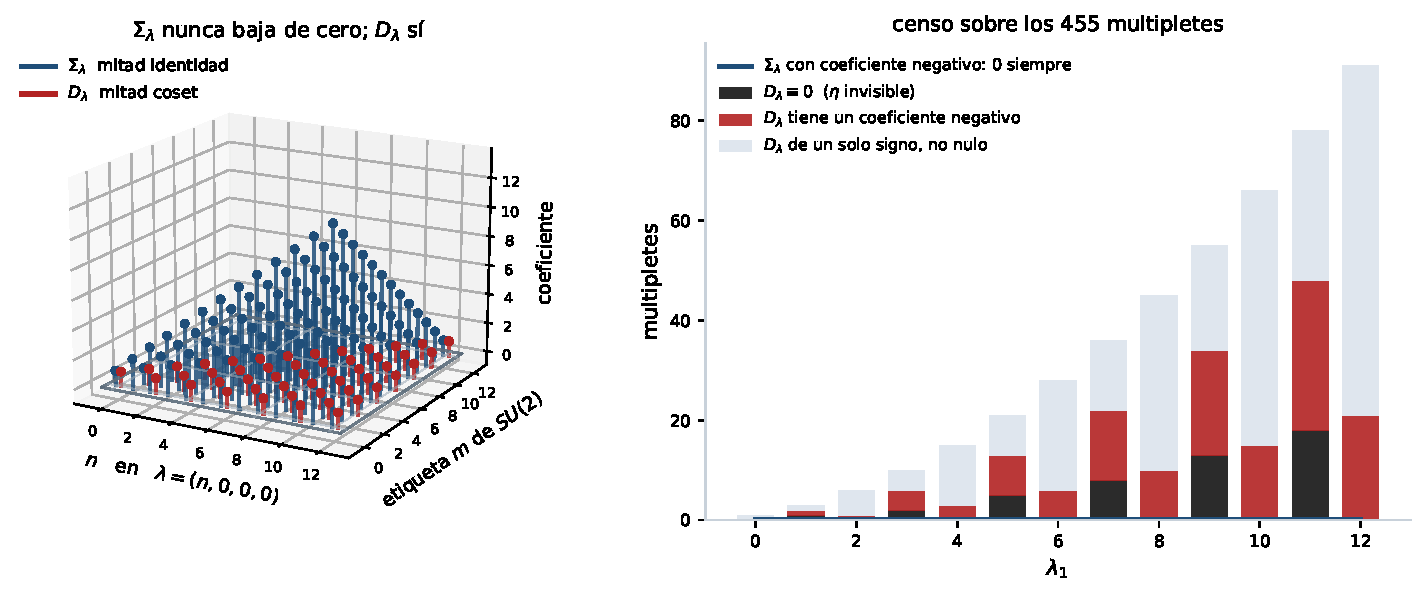
\includegraphics[width=\textwidth]{fig_positivity_es.pdf}
\caption{La asimetría de \eqref{eq:dimindex}, medida. \textbf{Izquierda:} las dos mitades
desarrolladas en caracteres de $SU(2)$ sobre la familia simétrica $\lambda=(n,0,0,0)$, que contiene
el $\mathbf{35}=(4,0,0,0)$ de AHMN. Cada tallo es un coeficiente, y el marco perfilado es el nivel
cero. Todo tallo azul queda por encima, porque los coeficientes de la mitad identidad son dimensiones
$n^+_m+n^-_m$; los rojos cuelgan por debajo, porque los de la mitad coset son índices $n^+_m-n^-_m$.
\textbf{Derecha:} el censo sobre los $455$ multipletes en rango, por $\lambda_1$ y de forma disjunta:
los que tienen $D_\lambda\equiv0$ (la clase ciega, $47$), aquellos cuyo $D_\lambda$ tiene un
coeficiente de cada signo ($134$), y el resto. La línea plana es el recuento de multipletes cuyo
$\Sigma_\lambda$ tiene un coeficiente negativo: es $0$ en todo $\lambda_1$, y por \eqref{eq:dimindex}
tiene que serlo. Generada por \texttt{make\_figure\_positivity.py}.}
\label{fig:posit}
\end{figure}

\subsection*{Por qué una mitad factoriza y la otra no puede}

Que $\Dl$ factorice siempre y $\Sig$ nunca no es una diferencia de grado, y la causa no es que un
alfabeto tenga una letra de más. Es que $\{1,-1\}$ es el conjunto completo de raíces cuadradas de la
unidad y $\{1,1\}$ no lo es. Pegando un par recíproco libre $\{z,z^{-1}\}$ a un bloque congelado $F$
y preguntando, por el criterio de Kronecker, si todo cero de $s_\lambda$ está en el círculo unidad
--- equivalentemente, si el carácter es un monomio por un producto de polinomios ciclotómicos:

\begin{center}\small
\rowcolors{2}{softgrey}{white}
\begin{tabular}{lrrrl}
\toprule
\rowcolor{hdrblue!14}bloque congelado $F$ & no nulos & todos los ceros en $|z|=1$ & proporción &
peor fallo\\
\midrule
$\mu_2=\{1,-1\}$ & $212$ & $212$ & $100\%$ & ---\\
$\{1,1\}$ & $241$ & $16$ & $6.6\%$ & $1.62$\\
$\mu_3$ & $124$ & $124$ & $100\%$ & ---\\
$\{1,1,1\}$ & $150$ & $3$ & $2.0\%$ & $2.73$\\
$\mu_4$ & $86$ & $86$ & $100\%$ & ---\\
$\{1,1,1,1\}$ & $125$ & $2$ & $1.6\%$ & $3.79$\\
\bottomrule
\end{tabular}
\end{center}

\noindent \emph{Sólo la segunda columna de esa tabla es nuestra, y la distinción importa.} Que un
bloque de raíces de la unidad fuerce una factorización es clásico y tiene una línea larga: Littlewood
y Richardson mostraron que la acción de Verschiebung sobre $s_\lambda$ se anula cuando el $t$-núcleo
es no vacío y por lo demás factoriza sobre el $t$-cociente; Lecouvey~\cite{Lecouvey} y
Ayyer--Kumari~\cite{AK} hicieron los casos simpléctico y ortogonal, caracterizando la no anulación
por particiones $z$-asimétricas mediante un estudio de conjuntos beta; Albion~\cite{Albion} los
embebe todos en una familia. \emph{Nuestro} alfabeto --- todas las raíces $t$-ésimas de la unidad
junto con un par recíproco libre --- no está en ninguno de ellos: los alfabetos de esa línea llevan
una variable libre en cada letra, y el nuestro lleva exactamente una. Así que las filas al $100\%$
están medidas aquí y no leídas de un teorema publicado, y en $t=2$ son el lugar de ceros de la forma
cerrada de la Parte~IV, con el estatus de ésta.

Lo nuevo aquí es el \textbf{control}: nadie tenía motivo para correr los bloques de letras repetidas,
porque allí no hay teorema que demostrar. Nosotros sí lo teníamos --- $\{1,1\}$ es la mitad identidad
de un potencial de Higgs --- y la respuesta es que no factorizan prácticamente nunca, y fallan de
forma grosera. Un cero fuera del círculo por $1.62$ en módulo no es un artefacto numérico, mientras
que los bloques de raíces de la unidad sólo fallan con una tolerancia de $10^{-7}$ y desviaciones del
orden de $5\times10^{-6}$, y pasan a $10^{-4}$ [\texttt{why\_one\_factors.py}].

\emph{Y el reparto de trabajo no es el que esta serie suponía.} Cuatro artículos se fueron a $\Dl$
porque tiene ceros que clasificar y $\Sig$ no los tiene, y la frase de arriba dice por qué. Pero no
tener ceros no es lo mismo que no llevar información, y resulta ser al revés: $\Sig$ \emph{por sí
solo} determina el multiplete salvo conjugación --- sus fibras sobre $969$ multipletes son
exactamente las órbitas $\{\lambda,\lambda^*\}$, y los singletes son exactamente los autoconjugados
(\S\ref{sec:scope}). Así que la mitad de winding par del potencial lleva la \emph{identidad} de la
materia, y la de winding impar lleva la \emph{condición de contorno}. La mitad que nadie minó es la
que dice qué es la materia.

La Figura~\ref{fig:zeros} es el mismo enunciado contado cero a cero en vez de polinomio a polinomio.

Dos consecuencias que conviene separar. \emph{Matemáticamente}, ``factoriza en tres caracteres de
$SU(2)$'' es el enunciado correcto sólo en $t=2$: en $t=3$ las piezas son ciclotómicas y \emph{no}
son caracteres de $SU(2)$ --- $\lambda=(2,1,0,0,0)$ da $z-1+z^{-1}$, el sexto polinomio ciclotómico.
El enunciado uniforme en $t$ es la localización de los ceros. \emph{Físicamente}, y ésta es la
lectura: \emph{la amplitud coset de un multiplete se anula sólo en fases de línea de Wilson
racionales}, porque sus ceros son raíces de la unidad en $z=e^{i\pi\theta}$; la amplitud identidad
tiene sus ceros enteramente fuera de la recta física. Una mitad está construida para anularse en
puntos especiales de la línea de Wilson y la otra no.

\begin{figure}[t]
\centering
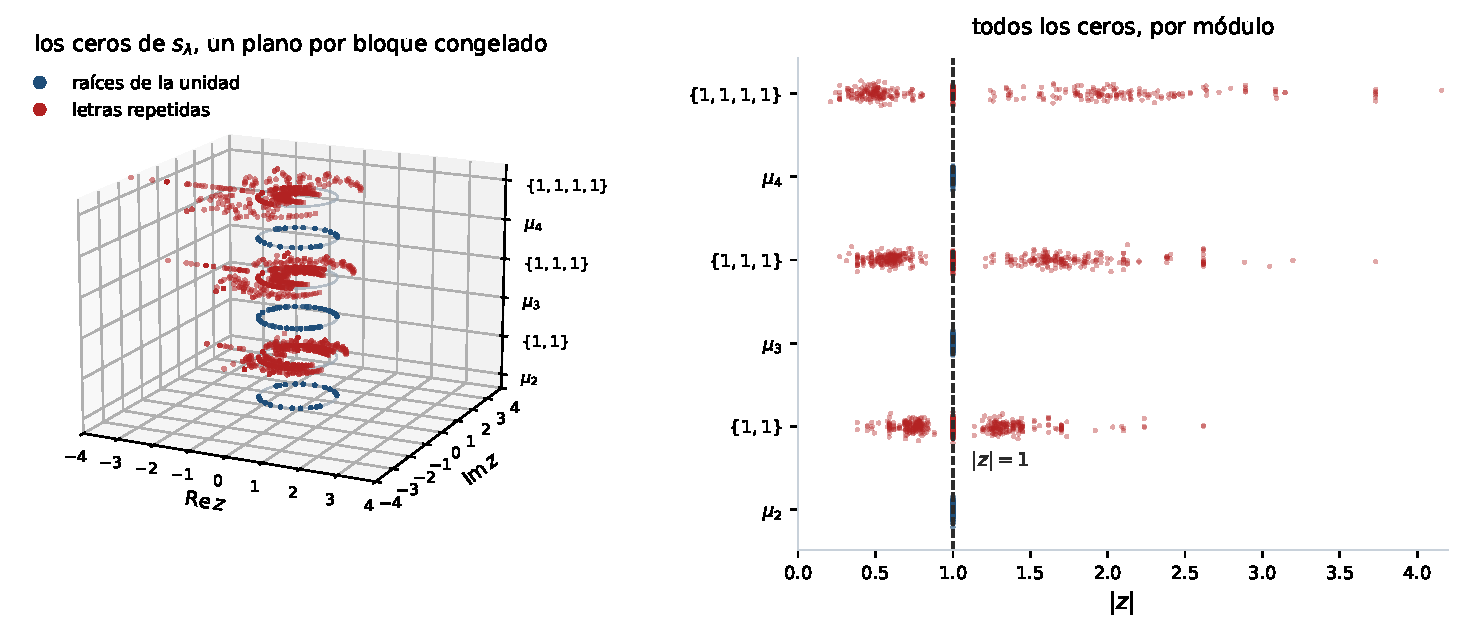
\includegraphics[width=\textwidth]{fig_zeros_es.pdf}
\caption{La misma dicotomía al nivel de ceros individuales y no de porcentajes. \textbf{Izquierda:}
el plano complejo $z$ apilado una vez por bloque congelado, con el círculo unidad dibujado en cada
capa. Todo cero de todo $s_\lambda$ construido sobre un bloque de raíces de la unidad está
\emph{sobre} su círculo; todo bloque de letras repetidas los dispersa fuera. \textbf{Derecha:} los
mismos puntos por módulo. Los bloques de raíces de la unidad son un único pico exactamente en $1$;
los otros se extienden hasta $|z|=2.618$, $3.732$ y $4.791$. Contando ceros en vez de polinomios:
$618$, $408$ y $218$ ceros para $\mu_2,\mu_3,\mu_4$, todos en $|z|=1$ hasta $10^{-4}$; y $51.6\%$,
$37.5\%$, $22.5\%$ para $\{1,1\}$, $\{1,1,1\}$, $\{1,1,1,1\}$. \emph{La mitad coset del potencial
está construida para anularse en fases racionales de la línea de Wilson; la mitad identidad no.}
Generada por \texttt{make\_figure\_zeros.py}.}
\label{fig:zeros}
\end{figure}

\subsection*{Las dos mitades son un solo operador, trazado dos veces}

Antes de la lectura, la identidad que la hace exacta y no evocadora. Sea
$\sigma=\mathrm{diag}(1,-1,1,1)$ --- la paridad de orbifold de la Parte~III --- y sea
$g_t=\mathrm{diag}(1,1,t,t^{-1})$ el elemento de línea de Wilson. Entonces
$\sigma\,g_t=\mathrm{diag}(1,-1,t,t^{-1})$: \emph{el alfabeto del coset es $\sigma$ por el alfabeto
identidad}, letra a letra. Así que las dos mitades de \eqref{eq:V} son

\begin{keyeq}
\begin{equation}\label{eq:tracepair}
\Sig(t)\;=\;\mathrm{Tr}_{V_\lambda}\big(g_t\big),
\qquad
\Dl(t)\;=\;\mathrm{Tr}_{V_\lambda}\big(\sigma\,g_t\big),
\end{equation}
\end{keyeq}

\noindent la \emph{traza} y la \emph{traza torcida por $\sigma$} del mismo elemento del grupo sobre
el mismo espacio [verificado: la identidad de alfabetos, y $\tfrac12(\Sigma\pm D)$ enteros no
negativos en toda carga sobre todos los multipletes en rango, $287$ comprobaciones, $0$ fallos,
\texttt{verify\_formulas.py}]. Todo en este artículo es consecuencia de leer un operador dos veces.
Una traza es una dimensión y no puede anularse; una traza torcida es un índice y sí puede. El signo
de contorno multiplica la torcida y nada más. La clase ciega es donde la graduación se equilibra. Y
la forma estándar en que este campo escribe su potencial a un bucle, $\{A+B(-1)^{k_2}\}$, es ese
mismo par: $A$ y $B$ son los recuentos de modos $\sigma$-pares y $\sigma$-impares, y $A\pm B$ son la
traza y la traza torcida. Tres artículos distintos~\cite{AHMN,HY,HHHK} escriben el giro que las
intercambia en tres vocabularios --- una condición de contorno antiperiódica,
$Qa\mapsto Qa+\tfrac12$, y $a\mapsto a-\beta$ --- y ninguno lo nombra como una sola operación.

\emph{El límite de ese lenguaje, enunciado para que no se lea como más de lo que es.} ``Traza
torcida'' es aquí contabilidad exacta y no un teorema del índice: lo que clasifica el lugar de
anulación es combinatoria del $2$-cociente y del conjunto beta (Parte~IV, y la línea que va de
Littlewood--Richardson a \cite{Lecouvey,AK,Albion}), no un índice analítico. Afirmamos la identidad
\eqref{eq:tracepair} y las consecuencias que de ella extraemos, y nada de teoría del índice.

\subsection*{La raíz de la asimetría: una dimensión y un índice}

Las dos mitades se comportan distinto, y la razón no es una metáfora sobre cancelaciones. Sea
$\sigma=\mathrm{diag}(1,-1,1,1)$ --- la paridad de orbifold de la Parte~III --- y sea $SU(2)_{34}$ el
subgrupo que actúa sobre las dos últimas coordenadas, cuyo toro es exactamente
$\mathrm{diag}(1,1,t,t^{-1})$. \emph{Conmutan}, porque actúan sobre coordenadas complementarias. Así
que $V_\lambda$ se descompone bajo $SU(2)_{34}\times\langle\sigma\rangle$, y escribiendo $n^\pm_m$
para la multiplicidad de la representación de espín $\tfrac m2$ dentro del autoespacio $\sigma=\pm1$,
los desarrollos de las dos mitades en caracteres de $SU(2)$, $\chi_m$, son

\begin{keyeq}
\begin{equation}\label{eq:dimindex}
\Sig \;=\; \sum_m \big(n^+_m+n^-_m\big)\,\chi_m ,
\qquad
\Dl \;=\; \sum_m \big(n^+_m-n^-_m\big)\,\chi_m .
\end{equation}
\end{keyeq}

\noindent El primer coeficiente es una \emph{dimensión} y el segundo es un \emph{índice}. Ésa es toda
la asimetría, y no es una elección de lenguaje: es comprobable, porque afirma que
$\tfrac12(\Sigma_\chi\pm D_\chi)$ son enteros no negativos. [Verificado sobre los $455$ multipletes en
rango: $0$ no enteros, $0$ negativos. Y medido: $\Sig$ tiene un coeficiente de $SU(2)$ negativo en
$0$ de $455$, mientras que $\Dl$ lo tiene en $134$ --- Figura~\ref{fig:posit}.]

Se siguen dos cosas, y la segunda es la que este artículo necesitaba.

\begin{corollary}\label{cor:balance}
$\lambda\in\mathcal Z$ si y sólo si $n^+_m=n^-_m$ para \emph{todo} $m$: la clase de anulación la
forman exactamente los multipletes en los que todo nivel de $SU(2)$ está equilibrado en paridad.
\end{corollary}

\noindent [Verificado: $47$ equilibrados por nivel, $47$ en $\mathcal Z$, $0$ discrepancias.] Esto
afina la Parte~IV, que muestra que el índice de paridad \emph{total} $n_+-n_-$ se anula en
$\mathcal Z$. Junto con el Corolario~\ref{cor:regime} la cadena cierra: que un solo número se anule
--- una traza conservada en un punto fijo --- fuerza el equilibrio en todo nivel de la descomposición.

Y le da a $\eta$ su significado en una frase. El signo de contorno multiplica la mitad coset, esto
es, el índice; un multiplete con los niveles equilibrados tiene índice cero en todo nivel, luego no
hay nada que el signo pueda multiplicar. \emph{La invisibilidad de la condición de contorno es el
equilibrio exacto de paridad del multiplete de materia.}

\medskip
El mismo enunciado en el lenguaje antiguo: sobre pesos, la componente identidad lleva
$m_\mu+m_{\mu^*}$, que es no negativo de modo que nada puede cancelar, y el coset lleva
$m_\mu-m_{\mu^*}$, que tiene signo de modo que la cancelación es posible. Por tanto:

\begin{center}
\fcolorbox{warmred!55}{warmred!5}{\begin{minipage}{0.88\textwidth}
\emph{Las contribuciones de winding par al potencial de Higgs no pueden anularse nunca. Las de
winding impar sí pueden, y lo hacen, para un conjunto de representaciones que la Parte~IV clasifica
en forma cerrada.}
\end{minipage}}
\end{center}

\noindent El criterio de anulación de la Parte~IV tiene por tanto una lectura física: dice \emph{qué
multipletes no contribuyen nada a la parte de winding impar del potencial de Higgs}. Todo en
\S\ref{sec:obs} es consecuencia de esa única frase, porque el signo de contorno vive exactamente en
esa parte.

La mitad identidad no colapsa a una sola caja, y el contraste es más agudo de lo que un recuento
sugiere. Sobre las $359$ particiones con a lo sumo cuatro filas y $|\lambda|\le16$, exactamente $5$
tienen $\Sig$ igual a un producto de a lo sumo tres caracteres de $\su2$ --- y esas cinco son
$(n,n,n,n)$ para $n=0,\dots,4$, cinco representantes-partición de la \emph{misma} irreducible de
$\su4$, el singlete, cada uno con $\Sig\equiv1$. \emph{Factorizaciones no triviales: ninguna.} Donde
$\Dl$ factoriza siempre, $\Sig$ no lo hace nunca [\texttt{verify\_formulas.py}, portado de la
comprobación original en Sage]. En la misma base de bloques, sin embargo, es una
\emph{superposición positiva} explícita de las mismas cajas,
\begin{equation}\label{eq:evenstack}
s_\lambda(1,1,t,t^{-1}) \;=\; \sum_{0\le q\le p\le\lambda_1}(p-q+1)\,B(p,q),
\qquad B(p,q)=\chi_{m_1}\chi_{m_2}\chi_{m_3},
\end{equation}
con $m_1=\lambda_1-\max(p,\lambda_2)$, $m_2=\min(p,\lambda_2)-\max(q,\lambda_3)$,
$m_3=\min(q,\lambda_3)-\lambda_4$, y un término descartado siempre que algún $m_i<0$ [verificado
$286/286$ en aritmética entera exacta, \texttt{verify\_formulas.py}], bajo el peso
$s_\nu(1,1)=p-q+1$, allí donde la mitad coset lleva el alternante $s_\nu(1,-1)$.

\emph{El rango de sumación en \eqref{eq:evenstack} no es una elección, y conviene decirlo porque un
rango no enunciado es una hipótesis escondida.} Como $\max(a,b)+\min(a,b)=a+b$, los tres índices de
bloque satisfacen
\begin{equation}\label{eq:degid}
m_1+m_2+m_3 \;=\; (\lambda_1-\lambda_4)-|p-\lambda_2|-|q-\lambda_3|
\end{equation}
[$0$ fallos en $674\,245$ pares]. Por \eqref{eq:degid} el sumando tiene soporte exactamente donde
$\lambda_1\ge\max(p,\lambda_2)\ge\min(p,\lambda_2)\ge\max(q,\lambda_3)\ge\min(q,\lambda_3)\ge\lambda_4$
--- una cadena de entrelazado cuyos huecos primero, tercero y quinto son $m_1,m_2,m_3$. Ese soporte es
finito y la condición $m_i\ge0$ lo impone por sí sola: sumar sobre $0\le p,q\le\lambda_1$, sobre
$[-15,\lambda_1{+}15]^2$ y sobre $[-40,\lambda_1{+}40]^2$ da la misma respuesta, $0$ fallos de $60$
multipletes cada vez; y de los $4104$ pares con los tres $m_i\ge0$ que aparecen en esas tres cajas,
exactamente $0$ tienen $q>p$, así que incluso $q\le p$ está implicado en vez de impuesto. No hay
constante de rango que acertar.

La \emph{positividad} de ese desarrollo no es un hallazgo y no la presentamos como tal:
$\mathrm{diag}(1,1,t,t^{-1})$ es el toro de un subgrupo $SU(2)$, luego $\Sig$ es una restricción de
$V_\lambda$ a ese subgrupo y sus multiplicidades son no negativas por la razón por la que lo son
todas las multiplicidades. Lo nuestro es el peso explícito $p-q+1$ y los índices de bloque que
recorre. De modo que todo el potencial a un bucle, ambas mitades, es una pila de cajas construidas a
partir de la única $G$ universal; la mitad coset colapsa a una sola caja porque sus pesos alternan, y
la mitad identidad no porque sus pesos son positivos.

Vale la pena enunciarlo como afirmación física y no sólo como identidad de funciones simétricas,
porque es el contenido operativo de toda la construcción:

\begin{center}
\fcolorbox{okgreen!55}{okgreen!5}{\begin{minipage}{0.88\textwidth}
\emph{Para cualquier multiplete, todo el potencial de Higgs a un bucle \eqref{eq:V} --- ambas
mitades --- es una suma con pesos enteros positivos de una única función universal evaluada en cargas
enteras leídas del diagrama de Young, con la mitad coset llevando delante un único signo global
$\zeta$. No hay que enumerar ningún espectro de Kaluza--Klein.}
\end{minipage}}
\end{center}

\noindent \emph{La afirmación hay que estrecharla, y aquí está el estrechamiento.} Un potencial a un
bucle general para esta clase de modelos no es nuevo: Haba y Yamashita~\cite{HY} dan uno para $\su N$
en 5D sobre $S^1/\ZZ_2$ en 2004, con fórmulas explícitas para el adjunto, el fundamental y los
tensores (anti)simétricos, y un método que ellos enuncian que se extiende a representaciones más
altas. Lo que no está en su artículo, ni en \cite{AHMN}, cuya ec.~(3.25), ni en \cite{KKKY}, cuyas
ecs.~(5.22)--(5.28) son listas ensambladas \emph{por representación} desde el desarrollo en modos, es
una fórmula \emph{cerrada en $\lambda$}: una única función universal cuyas cargas enteras se leen del
diagrama de Young de \emph{cualquier} irreducible, sin efectuar una descomposición representación por
representación. Eso, y sólo eso, es lo que se afirma aquí. La consecuencia es que el vacío
$\alpha_{\min}$, la curvatura en él y $\kappa_V$ pasan a ser calculables para contenido de materia
\emph{arbitrario} en vez de para el puñado cuyos espectros alguien ha escrito. Lo que uno luego
\emph{haga} con eso --- correrlo hacia adelante para predecir un espectro --- es asunto de la
Parte~VI, no de este artículo.

Dos límites honestos sobre esa afirmación, enunciados aquí y no después. La pila identidad puede
tener todavía una descripción más corta; nosotros no la tenemos. Y una forma cerrada para el
\emph{potencial} no es todavía una forma cerrada para la \emph{masa del Higgs}: la masa es la
curvatura en el mínimo verdadero, y hasta ahora sólo la curvatura en el origen está disponible en
forma cerrada. Minar la mitad identidad para el comportamiento dominante de $m_h$ está abierto, y es
la pieza de esta serie que menos hemos mirado.

\bridge{Han aparecido ya tres pares y los tres transforman igual: las dos componentes de $O(4)$, los
dos autoespacios de la involución asociada, y las dos paridades de modo del orbifold. ¿Tres
coincidencias, o un objeto visto tres veces?}

% ===================================================================
\section{Un solo $\ZZ_2$, visto tres veces}\label{sec:onez2}

Antes del ancla, conviene decir qué tienen en común los objetos de \S\ref{sec:two}, porque no son
tres coincidencias. Toda fórmula de este artículo es la misma transformada de Fourier sobre $\ZZ_2$
--- $\{f_+,f_-\}\mapsto\{f_++f_-,\,f_+-f_-\}$ --- leída a tres niveles distintos, y el contenido del
artículo es que los tres concuerdan.

\begin{center}\small
\rowcolors{2}{softgrey}{white}
\begin{tabular}{p{3.2cm} p{5.3cm} p{6.3cm}}
\toprule
\rowcolor{hdrblue!14}\textbf{nivel} & \textbf{el $\ZZ_2$} & \textbf{qué da la transformada}\\
\midrule
el grupo & $\pi_0(O(4))$: componente identidad frente a coset de reflexión & $\Sig$ y $\Dl$,
seleccionados por la paridad del winding\\
el multiplete & $\sigma=\mathrm{diag}(1,-1,1,1)$ actuando sobre $V_\lambda$ & $\Sigma_\chi=n^++n^-$
(una dimensión) y $D_\chi=n^+-n^-$ (un índice), \eqref{eq:dimindex}\\
el espectro & la paridad de orbifold de un modo de Kaluza--Klein & $A=\tfrac12(\Sigma+D)$ y
$B=\tfrac12(\Sigma-D)$, los coeficientes publicados de \S\ref{sec:anchor}\\
\bottomrule
\end{tabular}
\end{center}

\noindent La tercera fila es la que convierte el ancla, de una concordancia entre dos listas, en un
enunciado con mecanismo. AHMN obtienen su $A$ y su $B$ contando modos de Kaluza--Klein de cada
paridad de orbifold en cada carga. Lo que afirmamos es que $\Sig$ y $\Dl$ son las \emph{funciones
generatrices} de exactamente ese recuento, luego $A$ y $B$ no son constantes de ajuste: son números
de modos. Ése es un enunciado aritmético falsable --- $\tfrac12(\Sigma\pm D)$ tiene que ser un
\emph{entero no negativo} en toda carga, para todo multiplete --- y se cumple:

\begin{center}\small
\rowcolors{2}{softgrey}{white}
\begin{tabular}{lr}
\toprule
\rowcolor{hdrblue!14}\textbf{comprobación sobre los $455$ multipletes en rango} & \textbf{fallos}\\
\midrule
$A=\tfrac12(\Sigma+D)$ entero no negativo en toda carga & $0$\\
$B=\tfrac12(\Sigma-D)$ entero no negativo en toda carga & $0$\\
$\tfrac12(\Sigma_\chi\pm D_\chi)$ enteros no negativos (el nivel del multiplete) & $0$\\
\rowcolor{okgreen!14}$\Dl$ con coeficientes de $SU(2)$ de \textbf{ambos} signos & $\mathbf{0}$\\
\bottomrule
\end{tabular}
\end{center}

La última fila es consecuencia de la Parte~IV y es la más afilada de las cuatro. La forma cerrada de
la Parte~IV da $\Dl=\zeta\,\chi_{a_1}\chi_{a_2}\chi_{a_3}$ o $0$; un producto de caracteres de $SU(2)$
tiene multiplicidades de Clebsch--Gordan no negativas; por tanto

\begin{keyeq}
\begin{equation}\label{eq:onesign}
n^+_m-n^-_m \;=\; \zeta\cdot c_m,\qquad c_m\ge0\ \text{para todo } m .
\end{equation}
\end{keyeq}

\noindent \emph{El desequilibrio de paridad de un multiplete apunta en la misma dirección en todo
nivel de $SU(2)$}, y $\zeta$ --- que la Parte~IV identificó como el signo del índice de paridad total
--- es esa única dirección. El Corolario~\ref{cor:balance} es entonces inmediato en vez de
sorprendente: por \eqref{eq:onesign}, una suma de términos de un solo signo se anula sólo si se anula
cada término, de modo que un índice total nulo fuerza el equilibrio nivel a nivel. El
Corolario~\ref{cor:regime} es el mismo argumento en la otra base.

\bridge{Si la tercera fila de esa tabla es correcta, entonces los coeficientes publicados por otro
--- obtenidos contando modos, no con nada de esto --- tienen que \emph{ser} nuestros
$\tfrac12(\Sigma\pm D)$. Ésa es una afirmación sobre números que no produjimos nosotros, y es lo
siguiente que hay que comprobar.}

% ===================================================================
\section{Tres anclas: potenciales publicados, reproducidos}\label{sec:anchor}

Una afirmación estructural de este tipo no vale nada hasta que reproduce números que otro imprimió.
Una sola concordancia es una coincidencia que no se puede descartar, así que hay tres, elegidas para
compartir lo menos posible. Akamatsu, Hirose, Maru y Nago~\cite{AHMN} calculan el potencial a un
bucle de este modelo y lo escriben con coeficientes de la forma $\{A+B(-1)^{k_2}\}$. Bajo
\eqref{eq:alphabets} esa forma está forzada, y el diccionario queda fijado sin libertad alguna:
$k_2$ par selecciona $A+B$ y $k_2$ impar selecciona $A-B$, luego
\begin{keyeq}
\begin{equation}\label{eq:dict}
A \;=\; \tfrac12\big(\Sig+\Dl\big), \qquad B \;=\; \tfrac12\big(\Sig-\Dl\big).
\end{equation}
\end{keyeq}
Evaluado por carga (con el exponente dividido por dos) y comparado con sus valores impresos, sin
ajustar nada:

\begin{center}\small
\rowcolors{3}{softgrey}{white}
\begin{tabular}{c cc cc cc}
\toprule
\rowcolor{hdrblue!14}
& \multicolumn{2}{c}{nuestro} & \multicolumn{2}{c}{nuestro} &
\multicolumn{2}{c}{\textbf{AHMN ec.~(3.25)}}\\
\rowcolor{hdrblue!14}
carga & $\Sigma$ & $D$ & $A$ & $B$ & $A$ & $B$\\
\midrule
$2.0$ & $1$ & $1$ & $1$ & $0$ & $1$ & $0$\\
$1.5$ & $2$ & $0$ & $1$ & $1$ & $1$ & $1$\\
$1.0$ & $4$ & $2$ & $3$ & $1$ & $3$ & $1$\\
$0.5$ & $6$ & $0$ & $3$ & $3$ & $3$ & $3$\\
\bottomrule
\end{tabular}
\end{center}

\noindent Ocho números para el $\mathbf{35}=(4,0,0,0)$, exactos. Su ec.~(3.11), el adjunto gauge
$\mathbf{15}=(2,1,1,0)$, concuerda tras el giro $(-1)^{k_2}$ que \emph{ellos} enuncian en su texto
(condiciones de contorno antiperiódicas), que bajo \eqref{eq:dict} es precisamente
$A\leftrightarrow B$: el crudo $\{2:(0,1),\,1:(2,2)\}$ pasa a ser $\{2:(1,0),\,1:(2,2)\}$. Su
ec.~(4.1) es su propio $3\times(3.25)-(3.11)$, aquí rededucida como control interno. De regalo, las
dos comprobaciones de dimensión $\Sigma(1)=35$ y $\Sigma(1)=15$ salen bien. Doce números publicados,
nada ajustado [\texttt{ahmn\_anchor.py}, salida en \texttt{outputs/ahmn\_anchor.txt}].

Leída con \S\ref{sec:onez2}, la tabla dice más que ``los números concuerdan'': la columna $A$ es el
recuento de modos de paridad par en esa carga y $B$ el de los de paridad impar, que es como se
obtuvieron en primer lugar. El diccionario \eqref{eq:dict} es la transformada inversa de $\ZZ_2$, y
la razón de que no haga falta ajustar nada es que no hay nada que ajustar.

\subsection*{Una segunda ancla, elegida lo más distinta que supimos}

Un ancla sola es una coincidencia que no se puede descartar. La segunda es Haba y Yamashita~\cite{HY}:
otro grupo, otro número de dimensiones, otro orbifold y otra deducción --- ellos descomponen la
representación bajo el $SU(2)$ que selecciona el VEV de la línea de Wilson y leen los autovalores del
generador, donde nosotros leemos un diagrama de Young. Su ejemplo trabajado es $\su3$ sobre
$S^1/\ZZ_2$ con $P=P'=\mathrm{diag}(+,-,-)$, e imprimen cuatro cosas. Las cuatro salen de nuestro
recuento de modos sin ajustar nada [\texttt{hy\_anchor.py}]:

\begin{center}\small
\rowcolors{2}{softgrey}{white}
\begin{tabular}{lll}
\toprule
\rowcolor{hdrblue!14}su ecuación & qué dice & la nuestra\\
\midrule
(3.8) & cargas $(+1,-1,0,0,+\tfrac12,-\tfrac12,+\tfrac12,-\tfrac12)$ & multiconjunto idéntico\\
(3.2) & todo elemento de la base es $(+,+)$ o $(-,-)$, nunca mixto & idéntico\\
(3.9) & modos: $2$ en $|Q|=1$, $4$ en $|Q|=\tfrac12$, $2$ en $Q=0$ & idéntico\\
(3.10) & $V=\tfrac{C}{2}\sum_n n^{-5}\,[\cos 2na + 2\cos na]$ &
$[\cos 2na + 2\cos na]$\\
\bottomrule
\end{tabular}
\end{center}

\noindent Y su ec.~(3.11) merece una frase propia. Para $\eta=-1$ desplazan $Qa\mapsto Qa+\tfrac12$,
que es un factor $(-1)^n$ sobre la suma de windings --- eso es $A\leftrightarrow B$ en la notación de
\S\ref{sec:onez2}, y es \emph{el mismo giro} que AHMN enuncian para su sector gauge como condición de
contorno antiperiódica. Dos artículos independientes, dos vocabularios, una sola operación.

Una frase de método, porque estuvo a punto de entrar mal. Comparados de forma ingenua --- nuestros
caracteres contra sus coeficientes, término a término --- los números \emph{no} concuerdan, $0$ de
$4$. Es \eqref{eq:dict} lo que los hace concordar, y \eqref{eq:dict} es la afirmación física, no una
comodidad de ajuste. Una comparación rápida habría reportado una refutación.

\bridge{El diccionario aguanta contra los números impresos de tres artículos distintos. Lo que
todavía no dice es cuál de las dos mitades puede \emph{bloquear} la ruptura de la simetría
electrodébil --- y sólo una puede, por una razón aritmética y no dinámica.}

% ===================================================================
\section{Las dos mitades, y cuál puede bloquear}\label{sec:halves}

Las dos especializaciones son los autoespacios de la involución asociada $\mu\mapsto\mu^*$ de $O(N)$
sobre pesos: la componente identidad lleva la combinación simétrica $m_\mu+m_{\mu^*}$, que es no
negativa y no puede cancelar, y el coset lleva la antisimétrica $m_\mu-m_{\mu^*}$, que sí puede. La
lectura física es inmediata y es la razón por la que el criterio de anulación de la Parte~IV importa
aquí: \emph{la mitad identidad aporta siempre el signo que rompe la simetría electrodébil a la
curvatura en el origen, y la mitad coset es lo único que puede cancelarlo ahí} --- un enunciado
sobre el origen, no sobre $V(\alpha)$ globalmente, como explicita la advertencia bajo
\eqref{eq:crit}. Con el peso geométrico $\rho=7.5115$ para 6D sobre $T^2$, el criterio
cerrado
\begin{equation}\label{eq:crit}
\text{rompe}\iff \sum_i n_i\Big[\frac{2\,\dim_i\,C_2(i)}{\dim G}+\rho\,\varepsilon_i\,M_2\delta_i\Big] > 0
\end{equation}
reproduce el cálculo directo.

\subsection*{Por qué el índice pesa más que la dimensión, y cuánto}

El criterio \eqref{eq:crit} es una competición entre una dimensión y un índice, y el índice entra
pesado $\rho\approx7.5$ veces más por unidad de momento. Ese factor no es un acoplo y no está
ajustado; es geometría, y su origen es una línea de aritmética.

La curvatura en $\alpha_2$ pesa cada winding $k$ por $k_2^2$, así que el winding $k_2=0$ contribuye
\emph{exactamente nada} --- el sector identidad pierde gratis su capa más corta. Su capa siguiente es
$|k_2|=2$, el doble de larga, mientras que el sector coset arranca en $|k_2|=1$; y la suma de windings
decae como $|k|^{-2p}$, con $p=3$ para 6D. De modo que el sector coset se queda con la capa que domina
la suma:

\begin{center}\small
\rowcolors{2}{softgrey}{white}
\begin{tabular}{lrl}
\toprule
\rowcolor{hdrblue!14}capa $|k_2|$ & contribución a $p=3$ & \\
\midrule
$0$ & $0.00000$ & par --- ausente, aniquilada por el peso $k_2^2$\\
$1$ & $2.53718$ & impar --- el $95\%$ de toda la suma coset\\
$2$ & $0.29466$ & par --- el $83\%$ de toda la suma identidad\\
$3$ & $0.08727$ & impar\\
\bottomrule
\end{tabular}
\end{center}

\noindent luego $\rho=A_{\mathrm{impar}}/A_{\mathrm{par}}=2.65906/0.35400=7.5115$. El control que
podría haber falsado esta lectura hace lo contrario: quitar \emph{sólo} la capa $|k_2|=1$ manda
$\rho\to0.3443$, y el índice deja por completo de pesar más que la dimensión. Y $\rho$ es función
pura del decaimiento, y por tanto de la dimensión de la compactificación: $1.0060$ en $p=1.5$,
$7.5115$ en $p=3$, $35.5608$ en $p=4$, $676.8241$ en $p=6$.

\emph{El índice pesa más porque el winding más corto es impar.} Eso es todo, y significa que $\rho$
está fijado por la geometría y no elegido. También pone un límite a cuánto peso puede soportar
\eqref{eq:crit}: la base $\mathbf{60}$ de este modelo tiene $\rho$ crítico $6.4545$ frente a un
$7.5115$ real, así que un desplazamiento del $14.1\%$ en $\rho$ invierte su veredicto. Los veredictos
cerca de ese margen deben leerse como tales.

\medskip
Una advertencia que pertenece junto a \eqref{eq:crit} y no a una nota al pie: comprueba la
inestabilidad del \emph{origen}. Un contenido puede tener origen estable y un mínimo más bajo en otro
sitio --- el $\mathbf{45}$ lo tiene --- así que el criterio es local, no global.

La clase de anulación $\mathcal Z$ de la Parte~IV nombra por tanto exactamente la materia que no
tiene voz en el bloqueo: un multiplete así contribuye por su índice de Dynkin y por nada más.

\bridge{Así que una mitad del potencial puede anularse del todo, sobre una clase ya clasificada en
forma cerrada. La pregunta para la que existe este artículo es qué deja de ser observable cuando lo
hace.}

% ===================================================================
\section{Lo que el potencial puede ver}\label{sec:obs}

\subsection*{El signo, y qué es}

Cada multiplete de materia lleva un signo discreto de condición de contorno. En nuestras variables es
el giro por el determinante $\lambda\mapsto\lambda+(1,1,1,1)$, que es la \emph{misma} representación
irreducible de $\su4$ [verificado sobre $212$ particiones] y multiplica el carácter por $\det$:
trivial en la componente identidad, un signo en el coset. Así que $\eta\in\{\pm1\}$ actúa como
\begin{equation}\label{eq:etaact}
\eta:\quad (\Sig,\;\Dl)\;\longmapsto\;(\Sig,\;\eta\,\Dl),
\end{equation}
y el observable físico de un multiplete es el \emph{par} $(\Sig,\eta\Dl)$: dos multipletes con el
mismo par dan el mismo potencial en todo $\alpha$, luego el mismo vacío, las mismas masas y el mismo
$\kappa_V$.

Ese signo no es nuestro y tiene nombre. Haba, Hosotani y Kawamura~\cite{HHK} adjudican a cada campo
de materia dos signos $\eta_0,\eta_1\in\{\pm1\}$, uno por paridad de orbifold,
$\phi(x,-y)=\eta_0P_0\phi(x,y)$ y $\phi(x,R-y)=\eta_1P_1\phi(x,R+y)$; el volteo global
$(\eta_0,\eta_1)\to(-\eta_0,-\eta_1)$ es una redundancia que ellos mismos enuncian, y todo lo finito
del potencial depende del par sólo a través del producto. Nuestro $\eta$ es ese producto,
\begin{equation}\label{eq:etaname}
\eta \;:=\; \eta_0\eta_1 ,
\end{equation}
y \S\ref{sec:hhk} hace la identificación exacta en vez de terminológica.

\subsection*{El teorema}

\begin{theorem}\label{thm:main}
Para todo par $(\lambda,\eta)$,
\begin{keyeq}
\begin{equation}\label{eq:rel}
(\lambda,\eta)\;\sim\;\big(\lambda^*,\;\eta\,(-1)^{\lambda_1}\big)
\end{equation}
\end{keyeq}
es una identidad observacional: los dos pares dan el mismo $(\Sig,\eta\Dl)$ y por tanto el mismo
potencial en todo $\alpha$. Y $\eta$ es inobservable para $\lambda$ \emph{si y sólo si}
$\Dl\equiv0$ --- por la identidad de la Parte~IV, exactamente en su clase de anulación
$\mathcal Z$: para esos multipletes la condición de contorno no tiene consecuencia alguna que
ninguna medida de este sector de Higgs pueda ver.
\end{theorem}

\begin{proof}[Demostración de la relación]
Los dos alfabetos de \eqref{eq:alphabets} son estables bajo inversión, luego
$s_\lambda(A^{-1})=s_\lambda(A)$; $\lambda^*$ es el complemento de $\lambda$ en el rectángulo
$4\times\lambda_1$, luego la identidad clásica de complementación da
$s_{\lambda^*}(A)=\det(A)^{\lambda_1}s_\lambda(A)$; y $\det=+1$ en la componente identidad, $-1$ en
el coset. Por tanto $\Sigma_{\lambda^*}=\Sig$ siempre y $D_{\lambda^*}=(-1)^{\lambda_1}\Dl$, que es
\eqref{eq:rel} actuando sobre \eqref{eq:etaact}. Que $\eta$ sea inobservable cuando $\Dl\equiv0$ es
\eqref{eq:etaact} misma.
\end{proof}

El teorema dice que \eqref{eq:rel} \emph{es} una colisión y cuándo degenera. Que sea la \emph{única}
es un enunciado distinto, con otro estatus, y se enuncia por separado:

\begin{observation}[completitud --- verificada, no demostrada]\label{obs:complete}
Sobre el rango barrido, toda colisión observacional es una instancia de \eqref{eq:rel}: no hay dos
pares fuera de la relación que compartan un $(\Sig,\eta\Dl)$.
\end{observation}

\noindent El barrido es sobre las irreducibles de $\su4$ con $\lambda_1\le12$ y $\lambda_4=0$, en
aritmética entera exacta de Laurent [\texttt{fibre\_eta.py}, datos en
\texttt{outputs/fibre\_eta.json}]:

\begin{center}\small
\rowcolors{2}{softgrey}{white}
\begin{tabular}{lr}
\toprule
pares $(\lambda,\eta)$ & $910$\\
clases observacionales & $470$\\
tamaños de fibra & $56$ de tamaño $1$, $401$ de tamaño $2$, $13$ de tamaño $4$ --- nada más\\
\rowcolor{okgreen!14}\textbf{fibras no generadas por \eqref{eq:rel}} & $\mathbf{0}$\\
irreducibles en $\mathcal Z$ & $47$\\
irreducibles cuyo $\eta$ es inobservable & $47$, las mismas, por ningún otro mecanismo\\
\bottomrule
\end{tabular}
\end{center}

\noindent La Figura~\ref{fig:fibre} pone los tres casos uno al lado del otro. Las clases de tamaño
cuatro son los $13$ pares conjugados dentro de $\mathcal Z$, donde actúan tanto
$\lambda\leftrightarrow\lambda^*$ como $\eta\leftrightarrow-\eta$ y
$\{(\lambda,\pm),(\lambda^*,\pm)\}$ colapsa a un solo observable.

\begin{figure}[t]
\centering
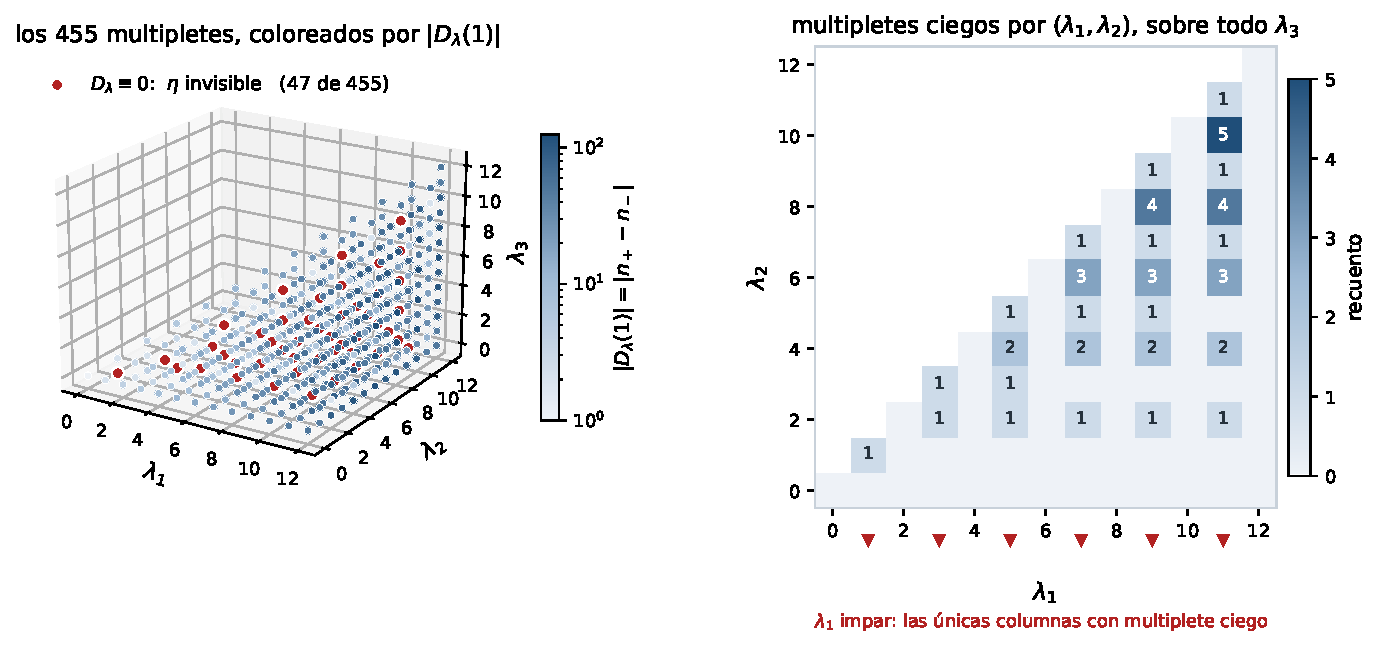
\includegraphics[width=\textwidth]{fig_blindclass_es.pdf}
\caption{La clase ciega, dibujada desde el barrido archivado. \textbf{Izquierda:} cada multiplete de
$\su4$ con $\lambda_1\le12$, $\lambda_4=0$, colocado en $(\lambda_1,\lambda_2,\lambda_3)$ y coloreado
por la magnitud $|D_\lambda(1)|=|n_+-n_-|$, el índice de paridad de la Parte~IV, sobre una rampa
logarítmica de un solo tono. Los $47$ multipletes de $\mathcal Z$ no llevan magnitud alguna y se
dibujan como clase propia: son aquellos cuyo signo de contorno $\eta$ no puede ver ninguna medida de
este sector de Higgs. \textbf{Derecha:} el mismo conjunto proyectado sobre $(\lambda_1,\lambda_2)$,
con cada celda contando los $\lambda_3$ que dan un multiplete ciego. La clase es una superficie
estructurada, no polvo disperso --- y la estructura se ve sin teoría ninguna: \emph{ningún multiplete
con $\lambda_1$ par es ciego jamás} (\S\ref{sec:count}). Generada por \texttt{make\_figures.py} desde
\texttt{outputs/fibre\_eta.json}; nada se recalcula para la figura.}
\label{fig:blind}
\end{figure}

\subsection*{Por qué los dos mecanismos son uno}

La relación \eqref{eq:rel} degenera --- mandando $(\lambda,\eta)$ a $(\lambda,-\eta)$ --- exactamente
cuando $\lambda$ es autoconjugada con $\lambda_1$ impar. Con $\lambda_4=0$, autoconjugada significa
$\lambda_2+\lambda_3=\lambda_1$, esto es $\lambda_i+\lambda_{5-i}=\lambda_1$ para todo $i$:
autocomplementaria de anchura $\lambda_1$. Con $\lambda_1$ impar eso es, palabra por palabra, la
rama~(b) del criterio de anulación de la Parte~IV. Así que la degeneración de la relación no es
información extra; es el mismo enunciado visto dos veces [verificado: $21$ de $21$ irreducibles de
ese tipo están en $\mathcal Z$, de $49$ autoconjugadas en rango].

\begin{figure}[t]
\centering
\begin{tikzpicture}[x=1cm,y=1cm,>=Latex]
\definecolor{cA}{RGB}{31,78,121}\definecolor{cB}{RGB}{0,140,54}\definecolor{cC}{RGB}{178,34,34}
% clase de tamano 2
\begin{scope}[shift={(0,0)}]
\node[anchor=south] at (1.6,1.5) {\small\textbf{genérico: $\lambda_1$ par}};
\node[draw,rounded corners,fill=softgrey,minimum width=1.5cm] (a1) at (0,0.7) {$(\lambda,+)$};
\node[draw,rounded corners,fill=softgrey,minimum width=1.5cm] (a2) at (3.2,0.7) {$(\lambda^*,+)$};
\node[draw,rounded corners,minimum width=1.5cm] (a3) at (0,-0.4) {$(\lambda,-)$};
\node[draw,rounded corners,minimum width=1.5cm] (a4) at (3.2,-0.4) {$(\lambda^*,-)$};
\draw[<->,cA,thick] (a1)--(a2); \draw[<->,cA,thick] (a3)--(a4);
\node[cA] at (1.6,-1.15) {\scriptsize dos clases de tamaño $2$};
\end{scope}
% clase de tamano 2, lambda1 impar
\begin{scope}[shift={(5.6,0)}]
\node[anchor=south] at (1.6,1.5) {\small\textbf{genérico: $\lambda_1$ impar}};
\node[draw,rounded corners,fill=softgrey,minimum width=1.5cm] (b1) at (0,0.7) {$(\lambda,+)$};
\node[draw,rounded corners,minimum width=1.5cm] (b2) at (3.2,0.7) {$(\lambda^*,+)$};
\node[draw,rounded corners,minimum width=1.5cm] (b3) at (0,-0.4) {$(\lambda,-)$};
\node[draw,rounded corners,fill=softgrey,minimum width=1.5cm] (b4) at (3.2,-0.4) {$(\lambda^*,-)$};
\draw[<->,cB,thick] (b1)--(b4); \draw[<->,cB,thick] (b3)--(b2);
\node[cB] at (1.6,-1.15) {\scriptsize el signo cruza: sigue siendo tamaño $2$};
\end{scope}
% Z
\begin{scope}[shift={(11.2,0)}]
\node[anchor=south] at (1.6,1.5) {\small\textbf{$\lambda\in\mathcal Z$}};
\node[draw,rounded corners,fill=cC!12,minimum width=1.5cm] (c1) at (0,0.7) {$(\lambda,+)$};
\node[draw,rounded corners,fill=cC!12,minimum width=1.5cm] (c2) at (3.2,0.7) {$(\lambda^*,+)$};
\node[draw,rounded corners,fill=cC!12,minimum width=1.5cm] (c3) at (0,-0.4) {$(\lambda,-)$};
\node[draw,rounded corners,fill=cC!12,minimum width=1.5cm] (c4) at (3.2,-0.4) {$(\lambda^*,-)$};
\draw[<->,cC,thick] (c1)--(c2);\draw[<->,cC,thick] (c3)--(c4);
\draw[<->,cC,thick] (c1)--(c3);\draw[<->,cC,thick] (c2)--(c4);
\node[cC] at (1.6,-1.15) {\scriptsize una clase de tamaño $4$: $\eta$ ha desaparecido};
\end{scope}
\end{tikzpicture}
\caption{La fibra de $(\lambda,\eta)\mapsto(\Sig,\eta\Dl)$, que es la clase de equivalencia
observacional. Las cajas sombreadas están en una misma clase. El signo $\eta$ sobrevive como
observable en los dos primeros paneles y desaparece en el tercero, y el tercero es exactamente
$\mathcal Z$: $D_\lambda\equiv0$ hace que $\eta$ actúe trivialmente allí, sobre los $47$ multipletes
de la clase. Una segunda ruta llega al mismo sitio --- cuando $\lambda$ es autocomplementaria de
anchura impar, \eqref{eq:rel} degenera e identifica por sí sola $(\lambda,+)$ con $(\lambda,-)$ --- y
no es independiente: son $21$ multipletes y los $21$ están dentro de los $47$. Ningún multiplete es
ciego a $\eta$ por ningún otro mecanismo. Recuentos sobre $\lambda_1\le12$: $56+401+13$ clases de
tamaño $1,2,4$ cubriendo los $910$ pares.}
\label{fig:fibre}
\end{figure}

\subsection*{Cuán grande es la clase ciega}\label{sec:count}

Como la Parte~IV clasifica $\mathcal Z$ en forma cerrada, el conjunto ciego se puede contar en vez de
estimar, y el recuento tiene más estructura de la que esperábamos. Para $\lambda_1$ fijo el barrido
es completo --- $\lambda_2$ y $\lambda_3$ recorren todo lo permitido --- así que son recuentos
exactos y no muestras:

\begin{center}\small
\rowcolors{2}{softgrey}{white}
\begin{tabular}{lccccccc}
\toprule
\rowcolor{hdrblue!12}
$\lambda_1$ & $1$ & $3$ & $5$ & $7$ & $9$ & $11$ & todo $\lambda_1$ par\\
\midrule
multipletes ciegos & $1$ & $2$ & $5$ & $8$ & $13$ & $18$ & \textcolor{warmred}{$0$}\\
$\lceil (k+1)^2/2\rceil$, $\lambda_1=2k{+}1$ & $1$ & $2$ & $5$ & $8$ & $13$ & $18$ & ---\\
\bottomrule
\end{tabular}
\end{center}

\noindent Los dos enunciados son consecuencia del criterio de la Parte~IV, y leerlos de él es un
argumento corto en vez de una deuda:

\begin{proposition}\label{prop:count}
Sea $\lambda=(\lambda_1,\lambda_2,\lambda_3,0)$. Entonces $\lambda\in\mathcal Z$ si y sólo si
\begin{enumerate}\itemsep1pt
\item[(a)] $\lambda_1$ impar, $\lambda_2$ par, $\lambda_3$ impar; \quad o
\item[(b)] $\lambda_1$ impar, $\lambda_2$ impar, $\lambda_3$ par y $\lambda_2+\lambda_3=\lambda_1$.
\end{enumerate}
Los dos casos son disjuntos. En particular $\lambda_1$ es \emph{impar} para todo
$\lambda\in\mathcal Z$, y para $\lambda_1=2k+1$
\[
\#\{\lambda\in\mathcal Z\}\;=\;\underbrace{\tfrac{k(k+1)}{2}}_{\text{(a)}}
\;+\;\underbrace{\lfloor k/2\rfloor+1}_{\text{(b)}}\;=\;\Big\lceil \tfrac{(k+1)^2}{2}\Big\rceil .
\]
\end{proposition}

\begin{proof}
El conjunto beta es $\beta=(\lambda_1+3,\lambda_2+2,\lambda_3+1,0)$, y la Parte~IV da
$D_\lambda\equiv0$ en exactamente dos situaciones: una clase de paridad de $\beta$ es vacía, o el
reparto es $2+2$ y $d_3=|a_1+a_2-b_1-b_2|=0$, donde $\chi_{-1}=0$.

Como $\beta_4=0$ es par, la clase par nunca es vacía, luego la primera situación es que la clase
impar sea vacía: $\lambda_1+3,\lambda_2+2,\lambda_3+1$ todos pares, que es (a).

Para la segunda, la clase par es $\{0,x\}$ con $x$ la única entrada par entre
$\beta_1,\beta_2,\beta_3$. Si $x=\beta_1$ entonces $\lambda_1$ es impar, la clase impar es
$\{\lambda_2+2,\lambda_3+1\}$, y $d_3=0$ se lee $\lambda_1+3=\lambda_2+\lambda_3+3$, que es (b). Si
$x=\beta_2$ entonces $d_3=0$ se lee $\lambda_2=\lambda_1+\lambda_3+2>\lambda_1$, en contradicción con
$\lambda_2\le\lambda_1$; si $x=\beta_3$ se lee $\lambda_3=\lambda_1+\lambda_2+4>\lambda_3$,
imposible. Los casos son disjuntos porque $\lambda_2$ es par en (a) e impar en (b).

El recuento en $\lambda_1=2k+1$. En (a), $\lambda_2=2j$ con $0\le j\le k$, y $\lambda_3$ impar con
$\lambda_3\le 2j$ deja $\lambda_3\in\{1,3,\dots,2j-1\}$, esto es $j$ valores; sumando da
$k(k+1)/2$. En (b), $\lambda_3=\lambda_1-\lambda_2$ está determinado y es automáticamente par, y
$\lambda_2\ge\lambda_3$ es $2\lambda_2\ge 2k+1$, es decir $\lambda_2\ge k+1$; los enteros impares en
$[k+1,2k+1]$ son $(k+1)-\lceil k/2\rceil=\lfloor k/2\rfloor+1$. Por último
$k(k+1)/2+\lfloor k/2\rfloor+1=\lceil (k+1)^2/2\rceil$, escribiendo $k=2m$ y $k=2m+1$ por separado.
\end{proof}

\noindent La Figura~\ref{fig:blind} dibuja la clase que la proposición cuenta, y su panel derecho es
el enunciado de paridad hecho visible: las columnas pobladas son exactamente las impares.

\noindent [Verificado con independencia de la demostración, sobre los $2925$ multipletes con
$\lambda_1\le24$: la caracterización discrepa del cálculo exacto de $D_\lambda$ en $0$ casos, las dos
ramas son disjuntas, y el total de cada rama se predice por separado --- rama~(a) $286$ contra $286$
medidos, rama~(b) $42$ contra $42$.]

\subsection{La proposición está verificada por máquina, y desciende del certificado de la Parte~III}
\label{sec:lean}

La Proposición~\ref{prop:count} está certificada en Lean~4~\cite{Lean4}
(\texttt{GHUBlindCount.lean}, Tabla~\ref{tab:leanV}). Lo relevante no es que un argumento de recuento
se haya vuelto a teclear en un asistente de demostración; es \emph{dónde empieza el certificado}. La
Parte~III ya lleva un ladrillo verificado por máquina, \texttt{NotchCentreCharge.lean}, cuyo teorema
principal es el criterio de anulación en etiquetas de Dynkin,
\[
N\,a\,b\,c=0\;\Longleftrightarrow\;\mathrm{Impar}\,b\wedge\big((\mathrm{Impar}\,a\wedge\mathrm{Impar}\,c)\vee a=c\big),
\]
demostrado por un desarrollo de Laplace honesto sobre $\mathbb{Z}[T;T^{-1}]$ sin ningún
\texttt{decide} sobre el determinante. La proposición de la Parte~V está enunciada en coordenadas de
partición, y el paso entre ambas es la sustitución $a=\lambda_1-\lambda_2$, $b=\lambda_2-\lambda_3$,
$c=\lambda_3$. Esa sustitución es exactamente el paso en el que un artículo de este tipo se tuerce en
silencio, así que es el paso que certificamos primero: \texttt{blind\_iff\_N\_zero} cierra el
circuito, y el recuento es por tanto un teorema \emph{sobre el determinante}, no sobre un predicado
que inventamos para poder contarlo.

También resuelve, de propina, algo que la serie nunca había comprobado mecánicamente. La
demostración de la Proposición~\ref{prop:count} de arriba lee las dos ramas del criterio de la
\emph{Parte~IV} --- las clases de paridad del conjunto beta y el reparto $2{+}2$ con $d_3=0$ ---
mientras que \texttt{blind\_iff\_notch} demuestra que esas dos mismas ramas equivalen al criterio de
la \emph{Parte~III} en etiquetas de Dynkin. Los dos artículos describen por tanto un mismo conjunto,
y la identificación está ahora verificada por máquina en vez de supuesta. Se suponía desde la
Parte~IV.

Antes de escribir una línea de Lean, el diccionario se barrió en Python sobre las $39711$ particiones
con $\lambda_1\le 60$, con $0$ discrepancias --- y, porque un control que no puede fallar no es un
control, el mismo barrido se corrió contra un diccionario corrompido a propósito ($c:=b$), que
rechaza sobre $5200$ particiones.

\begin{table}[t]
\centering\small
\begin{tabular}{p{5.6cm}p{8.5cm}}
\toprule
\rowcolor{hdrblue}
\textcolor{white}{Teorema en Lean}\newline\textcolor{white}{(\texttt{GHUBlindCount.lean})} &
\textcolor{white}{contenido}\\
\midrule
\texttt{blind\_iff\_notch} &
el diccionario: sobre $\lambda_1\ge\lambda_2\ge\lambda_3$, las ramas (a)/(b) son el criterio de
Dynkin\\
\midrule
\rowcolor{softgrey}
\texttt{blind\_iff\_N\_zero} &
$\lambda\in\mathcal Z\leftrightarrow N(\lambda_1{-}\lambda_2,\lambda_2{-}\lambda_3,\lambda_3)=0$
--- el puente con \texttt{NotchCentreCharge.lean}\\
\midrule
\texttt{blind\_l1\_odd} &
$\lambda\in\mathcal Z\Rightarrow\lambda_1$ impar; ningún multiplete con $\lambda_1$ par es ciego
jamás\\
\midrule
\rowcolor{softgrey}
\texttt{card\_shellA}, \texttt{card\_shellB} &
rama~(a) $=$ los pares estrictos $q<p\le k$, rama~(b) $=$ el intervalo $m\le\lfloor k/2\rfloor$;
(a) se enuncia duplicada, $2\,\#(\mathrm a)=(k{+}1)k$, de modo que en la demostración no entra
ninguna división sobre $\mathbb N$\\
\midrule
\texttt{card\_shell} &
$\#\{\lambda\in\mathcal Z:\lambda_1=2k{+}1\}=\lceil(k+1)^2/2\rceil$ --- la
Proposición~\ref{prop:count}\\
\bottomrule
\end{tabular}
\caption{El núcleo de la Parte~V verificado por máquina, lado materia. Todos los enunciados están
libres de \texttt{sorry} y dependen sólo de \texttt{propext}, \texttt{Classical.choice},
\texttt{Quot.sound}. La paridad de $\lambda_2$ es lo que parte la capa en las dos ramas, de modo que
la división en casos de la demostración del artículo y la de la demostración en Lean son la misma.
El lado geometría --- el censo de \S\ref{sec:hhk}, Proposición~\ref{prop:census} --- es un segundo
fichero, \texttt{GHUCosetCensus.lean}, con el mismo estatus y los mismos tres axiomas.}
\label{tab:leanV}
\end{table}

\paragraph{Dónde se detiene el certificado, exactamente.} La cadena está verificada por máquina desde
el determinante bialternante en adelante. \emph{No} lo está de vuelta hasta el carácter: la
identificación $D_\lambda(t)=s_\lambda(1,-1,t,t^{-1})=N/V$ es la definición bialternante clásica de
una función de Schur, usada aquí como entrada clásica, junto con $V\ne0$ (que \emph{sí} está
certificado, como \texttt{V\_ne\_zero}). Esa frontera no es cuestión de esfuerzo: Mathlib~\cite{Mathlib}
no tiene funciones de Schur en absoluto --- lleva \texttt{YoungDiagram} y
\texttt{SemistandardTableau}, y sus tres ficheros con el nombre de Schur son el lema de Schur,
Schur--Zassenhaus y el complemento de Schur. Formalizar
$s_{\lambda^*}(A)=\det(A)^{\lambda_1}s_\lambda(A)$, la identidad de complementación sobre la que se
apoya el Teorema~\ref{thm:main}, exigiría construir antes esa teoría, y no lo afirmamos. El
Teorema~\ref{thm:main} está por tanto demostrado pero no certificado; la
Proposición~\ref{prop:count} está ambas cosas.

\subsection*{Un paso más allá de un solo multiplete, y sale gratis}

El certificado se detiene ahí; el \emph{enunciado} no se detiene en un solo multiplete, y el paso más
allá cuesta una línea. Un contenido físico es un multiconjunto
$\{(\lambda_i,\eta_i,n_i)\}$ con multiplicidades $n_i>0$ y el observable es la suma, de modo que dos
contenidos podrían colisionar todavía por una cancelación que ningún par de multipletes hace. La
mitad de esa posibilidad se cierra en una línea. Escribiendo $\zeta_i$ para el signo de la forma
cerrada de la Parte~IV en $\lambda_i$, llamamos $\eta_i\zeta_i$ el \emph{signo efectivo} de ese
multiplete.

\begin{proposition}[signos coherentes]\label{prop:frust}
Si todos los multipletes no ciegos de un contenido llevan el mismo signo efectivo, entonces
$\sum_i n_i\,\eta_i D_{\lambda_i}\equiv0$ si y sólo si cada $\lambda_i$ es ciego por sí mismo.
\end{proposition}

\begin{proof}
La forma cerrada de la Parte~IV da $D_{\lambda_i}=\zeta_i P_i$ con $P_i$ de coeficientes no
negativos, luego $\eta_iD_{\lambda_i}=(\eta_i\zeta_i)P_i$. Si los signos efectivos comparten un
valor $\varepsilon$, la suma es $\varepsilon\sum_i n_iP_i$, una suma de términos de un solo signo con
pesos positivos, y se anula sólo si se anula cada $P_i$.
\end{proof}

\noindent Así que \textbf{la ceguera colectiva exige frustración de signos}: un contenido que no sea
ciego término a término sólo puede volverse ciego si lleva \emph{ambos} valores de $\eta_i\zeta_i$.
Esto no clasifica el caso frustrado --- eso es un problema de núcleo entero y es el artículo
siguiente --- quita la mitad estructuralmente simple, y lleva el estatus de la identidad de la
Parte~IV, sobre la que descansa la propiedad de un solo signo.

\subsection*{Qué afirmaba esta sección en un borrador anterior, y por qué estaba mal}

La primera versión de esta sección decía: \emph{la mitad coset es lo único observable de este modelo
que puede ver la conjugación de carga}. Eso es falso, y está contradicho en letra impresa. Kawamura,
Kodaira, Kojima y Yamashita~\cite{KKKY} escriben, sobre la representación conjugada, en su \S5.1,
``which is equivalent with the one of $\mathbf 4$. This holds for any representation'' --- y en su
formalismo es una línea, puesto que su potencial es una suma de cosenos y la conjugación cambia el
signo de las cargas. La conjugación de carga es aquí invisible \emph{sin condiciones}.

El signo $(-1)^{\lambda_1}$ de \eqref{eq:rel} es real; de lo que habla es de $\eta$. Como $U_6$ tiene
$\det=-1$ no está en $\su4$, luego ``el carácter de $\bar R$ en $U_6$'' no queda definido por $\su4$
solo: depende de qué extensión del multiplete al grupo generado por $\su4$ y el elemento que voltea
el determinante se elija, y las dos extensiones naturales difieren exactamente en $\det^{\lambda_1}$.
Esa elección es la condición de contorno. El enunciado que sobrevive es el
Teorema~\ref{thm:main}, y es más afilado que el que murió.

\bridge{El teorema está formulado en nuestra propia maquinaria, que es exactamente la condición bajo
la cual una afirmación no ha pasado puerta alguna. Dicho en el lenguaje que el campo usa desde 2004,
¿sobrevive --- y sigue siendo un enunciado sobre un solo modelo hexadimensional?}

% ===================================================================
\section{El mismo enunciado en las variables del campo}\label{sec:hhk}

El Teorema~\ref{thm:main} está formulado en nuestra maquinaria. No tiene por qué estarlo, y la
traducción hace más que renombrar cosas: muestra que el enunciado es una propiedad de la
clasificación pentadimensional de condiciones de contorno y no del modelo particular de
\S\ref{sec:anchor}.

Haba, Hosotani y Kawamura~\cite{HHK} clasifican las condiciones de contorno de la teoría gauge
$\su N$ sobre $S^1/\ZZ_2$ por los tamaños de bloque $[p;q,r;s]$ de las dos matrices de paridad
conmutantes $P_0,P_1$, demuestran que toda clase de equivalencia tiene un representante diagonal, y
cuentan las clases: $(N+1)^2$. Para el fundamental, el antisimétrico de segundo rango y el adjunto
tabulan (su ec.~(3.20)) las multiplicidades $N^{(\varepsilon_0,\varepsilon_1)}_{\mathrm{rep}}$ de
vectores de la base por su paridad $(P_0,P_1)$. Esas tablas son tres caracteres disfrazados:

\begin{proposition}\label{prop:three}
Para cualquier representación de $\su N$ y cualquier par conmutante de paridades $(P_0,P_1)$,
\begin{keyeq}
\begin{equation}\label{eq:threechar}
N^{(\varepsilon_0,\varepsilon_1)}
=\tfrac14\Big[\dim+\varepsilon_0\,\chi(P_0)+\varepsilon_1\,\chi(P_1)
+\varepsilon_0\varepsilon_1\,\chi(P_0P_1)\Big].
\end{equation}
\end{keyeq}
\end{proposition}

\noindent La Figura~\ref{fig:simplex} dibuja estos tres caracteres sobre todo el espacio de
condiciones de contorno, y muestra que cada uno lo estratifica en una dirección distinta. La
ecuación~\eqref{eq:threechar} es la traza del proyector
$\frac14(1+\varepsilon_0P_0)(1+\varepsilon_1P_1)$, y está verificada contra su tabla impresa sobre
todo $[p;q,r;s]$ hasta $N=8$: $1470$ casos, $0$ discrepancias con la ec.~(3.20) y $0$ con
\eqref{eq:threechar} [\texttt{hhk\_bridge.py}, salida en \texttt{outputs/hhk\_bridge.txt}]. Es
elemental, y queda registrada aquí como puente y no como descubrimiento: lo que compra es que los
tres números de la derecha son la \emph{única} manera en que entra una condición de contorno, para
toda representación y no sólo para las tres que están tabuladas.

Esos tres números tampoco son nuevos, y el lector debe conocer aquí a sus dueños. Takeuchi e
Inagaki~\cite{TI1,TI2} observaron que una transformación gauge que conecta condiciones de contorno
actúa sobre la matriz de rotación en un punto fijo por conjugación con $\Omega$ \emph{evaluado en ese
punto fijo} --- una constante --- de modo que la traza allí es invariante por ciclicidad, y llaman a
las identidades resultantes \emph{leyes de conservación de la traza}. Con ellas clasifican las clases
de equivalencia sobre $S^1/\ZZ_2$, $T^2/\ZZ_3$ y $T^2/\ZZ_m$ ($m=2,3,4,6$) sin escribir jamás una
transformación gauge, recuperando los recuentos y exhibiendo clases no diagonales. Su argumento es
ciego a la representación, luego $\chi_R$ en cada matriz de rotación de punto fijo es un invariante
de clase para \emph{toda} $R$; nada de eso lo reclamamos. La Proposición~\ref{prop:three} es el
recuento del proyector, un uso distinto de los mismos tres números, y ambos se encuentran en
\S\ref{sec:interp}.

\begin{figure}[t]
\centering
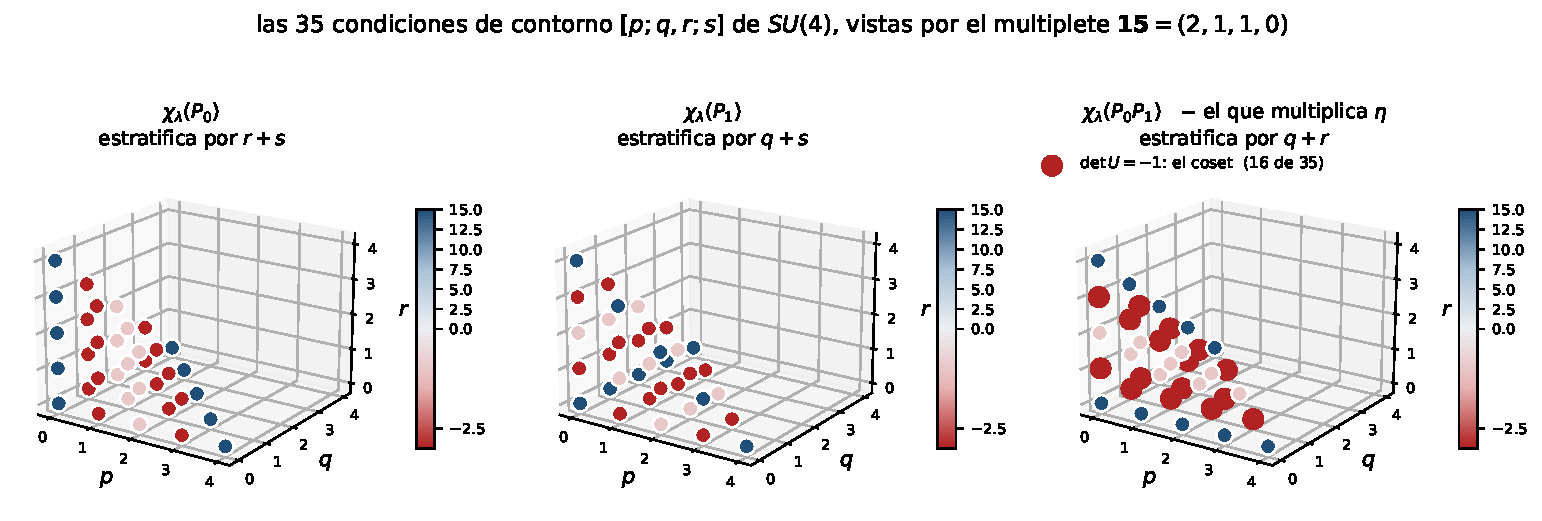
\includegraphics[width=\textwidth]{fig_simplex_es.pdf}
\caption{La Proposición~\ref{prop:three}, dibujada. Una condición de contorno de $\su4$ sobre
$S^1/\ZZ_2$ son cuatro enteros no negativos $[p;q,r;s]$ que suman $4$, así que el conjunto de ellas
\emph{es} un símplex con $35$ puntos; cada uno se coloca en $(p,q,r)$, con $s$ implícito. Los tres
paneles colorean el mismo símplex por los tres caracteres de \eqref{eq:threechar}, evaluados en el
adjunto gauge. El trabajo del color es la polaridad, así que la rampa es divergente con punto medio
neutro. \textbf{Cada carácter estratifica el símplex en una dirección distinta} --- $\chi(P_0)$
depende de los tamaños de bloque sólo por $r+s$, $\chi(P_1)$ por $q+s$, y $\chi(P_0P_1)$ por $q+r$;
las tres estratificaciones están verificadas, no afirmadas, en \texttt{make\_figure\_simplex.py}. El
tercer panel es el que importa aquí: es el carácter que multiplica el signo de contorno $\eta$, y los
puntos anillados son las $16$ condiciones de contorno con $\det U=-1$, el coset de reflexión --- el
único lugar de esta imagen donde $\eta$ puede actuar siquiera.}
\label{fig:simplex}
\end{figure}

Encender los signos de contorno manda $(P_0,P_1)\mapsto(\eta_0P_0,\eta_1P_1)$, luego
$\varepsilon_i\mapsto\eta_i\varepsilon_i$ en \eqref{eq:threechar}. Dos consecuencias se siguen por
inspección, y las dos están verificadas por barrido ($N\le6$, todos los $[p;q,r;s]$, tres
representaciones, $615$ casos, $0$ violaciones cada una):
\begin{enumerate}\itemsep2pt
\item $(\eta_0,\eta_1)\to(-\eta_0,-\eta_1)$ permuta las cuatro multiplicidades por
$(\varepsilon_0,\varepsilon_1)\to(-\varepsilon_0,-\varepsilon_1)$. Ésta es su propia frase debajo de
la ec.~(4.3), aquí como identidad: el volteo global es una redundancia.
\item La parte finita de su potencial usa sólo las sumas por pares $N^{(++)}+N^{(--)}$ y
$N^{(+-)}+N^{(-+)}$ (su $N_v$ en la ec.~(3.25), y las ecs.~(4.11)--(4.13)), y éstas son
$\frac12[\dim\pm\eta_0\eta_1\chi(P_0P_1)]$: dependen de los signos de contorno \emph{sólo} a través
del producto $\eta=\eta_0\eta_1$, y distinguen sus dos valores exactamente cuando
$\chi(P_0P_1)\neq0$.
\end{enumerate}
El signo individual $\eta_0$ sobrevive sólo en su término $N_\xi$, y $\xi$ es la cantidad divergente
que ellos mismos declaran incomparable entre clases de equivalencia. Todo lo finito ve el producto.
Por eso \eqref{eq:etaname} es una definición y no una aproximación.

Así que $\eta$ es invisible a un multiplete precisamente cuando el carácter en el elemento de winding
$U=P_0P_1$ se anula. Para $\su4$, $\det U=(-1)^{q+r}$, luego $U$ está en el coset de reflexión
exactamente cuando $q+r$ es impar --- $16$ de las condiciones de contorno --- y $U$ tiene entonces
sólo dos espectros, $\mathrm{diag}(1,1,1,-1)$ y $\mathrm{diag}(-1,-1,-1,1)$, la clase de conjugación
de la matriz de paridad $P_0$ de la Parte~III. Por tanto $\chi_\lambda(U)=s_\lambda(1,1,1,-1)=\Dl(1)$
y el Teorema~\ref{thm:main} se lee, en sus variables: \emph{$\eta_0\eta_1$ es invisible a $\lambda$ si
y sólo si $\chi_\lambda(U)=0$.}

\subsection{La línea de Wilson interpola las leyes de conservación de la traza}\label{sec:interp}

Las dos lecturas se encuentran, y el punto de encuentro es la frase más afilada que sabemos decir
sobre nuestro propio objeto. Una ley de conservación de la traza es un número: el carácter en una
matriz de rotación de punto fijo. Nuestro $\Dl$ es una \emph{función} de la fase de línea de Wilson,
y en $t=1$ es $\chi_\lambda(\mathrm{diag}(1,1,1,-1))$ --- el carácter en la matriz de paridad de la
Parte~III, esto es, exactamente una ley de conservación de la traza para la representación $\lambda$.
Así que las dos especializaciones de Schur de \eqref{eq:SigD} interpolan las trazas conservadas: los
invariantes de~\cite{TI1,TI2} son los extremos, y la fase de línea de Wilson es lo que corre entre
ellos. El teorema de \S\ref{sec:obs} dice entonces que el signo de contorno es invisible exactamente
donde esa función interpoladora es idénticamente nula --- y el corolario de abajo dice que eso ya
queda decidido en el extremo.

\subsection*{Una diferencia de régimen que resulta no serlo}

Sus fórmulas se evalúan a fase de línea de Wilson nula, donde el signo multiplica el número $\Dl(1)$;
la nuestra vive en una fase dinámica, donde multiplica el polinomio $\Dl(t)$. A priori $\Dl(1)=0$ es
la condición más débil y debería definir una clase estrictamente mayor de multipletes ciegos. No lo
hace.

\begin{corollary}\label{cor:regime}
$\Dl(1)=0\iff\Dl\equiv0$. El signo de la condición de contorno es invisible a fase de línea de Wilson
nula si y sólo si es invisible a toda fase, y ambas condiciones son $\mathcal Z$.
\end{corollary}

\begin{proof}
La forma cerrada de la Parte~IV da $\delta(m)=\zeta\cdot(\text{no negativo})$ con un único signo
global $\zeta$, de modo que todos los coeficientes de $\Dl=\sum_m\delta(m)t^m$ llevan el mismo signo;
una suma de términos de un solo signo se anula sólo si se anula cada término.
\end{proof}

\noindent En el lenguaje de \S\ref{sec:interp}: \emph{una sola traza conservada controla toda la
función interpoladora}, y lo hace porque la forma cerrada de la Parte~IV da a los coeficientes un
solo signo --- de modo que este corolario lleva el estatus de esa identidad, y ninguno mayor.

\noindent [Verificado sobre las $455$ irreducibles en rango: $0$ tienen coeficientes de ambos signos;
$\Dl(1)=0$ en $47$ y $\Dl\equiv0$ en las mismas $47$, con $0$ en una clase y no en la otra.]

La consecuencia práctica es que el teorema se puede citar a un lector pentadimensional y a uno
hexadimensional sin cambiar una palabra.

\subsection*{Qué es de ellos}

Dicho sin rodeos, porque el barrio es suyo: la clasificación $[p;q,r;s]$, la relación de equivalencia
$[p;q,r;s]\sim[p-1;q+1,r+1;s-1]$, el recuento $(N+1)^2$, el teorema del representante diagonal, el
potencial genérico a un bucle a fase de línea de Wilson nula, y la redundancia
$(\eta_0,\eta_1)\sim(-\eta_0,-\eta_1)$ están todos en~\cite{HHK}. También lo está una ceguera del
potencial: observan que su ec.~(4.13) ``is a function of $q+r$ only'' y ``does not select unique
$[p;q,r;s]$'', y cierran el artículo diciendo que el problema de la arbitrariedad sigue sin resolver
porque ``there remains a degeneracy among the theories of the lowest energy density''. Esa
degeneración está del lado de las \emph{etiquetas} de la condición de contorno. La nuestra está del
lado del \emph{contenido} de materia --- qué multipletes no pueden ver $\eta$ --- y las dos son
complementarias, del mismo espíritu, y no el mismo enunciado. Lo que se añade aquí es la
Proposición~\ref{prop:three} para representaciones generales, donde ellos tabulan tres a mano, y la
identificación en forma cerrada de la clase ciega.

\subsection*{Cuándo tiene un modelo sector de índice siquiera, y con qué frecuencia}

La raíz de \S\ref{sec:spine} es un test, y es un test sobre el \emph{embebido} y no sobre la materia:
existe sector coset si y sólo si $\det P_0\neq\det P_1$. En las etiquetas $[p;q,r;s]$ eso es
$\det U=(-1)^{q+r}$, y la paridad de $q+r$ es un invariante de clase --- el movimiento de
equivalencia manda $q+r\mapsto q+r+2$. Así que la pregunta se puede
contar, no sólo plantear:

\begin{center}\small
\rowcolors{2}{softgrey}{white}
\begin{tabular}{rrrr}
\toprule
\rowcolor{hdrblue!14}$N$ & clases $(N+1)^2$ & con sector de índice & sin él\\
\midrule
$2$ & $9$ & $4$ & $5$\\
$3$ & $16$ & $8$ & $8$\\
$4$ & $25$ & $12$ & $13$\\
$5$ & $36$ & $18$ & $18$\\
$\vdots$ & & & \\
$10$ & $121$ & $60$ & $61$\\
\bottomrule
\end{tabular}
\end{center}

\noindent El patrón es exacto, y es un teorema y no un barrido. El movimiento deja intacto el par
$(p+q,\,q+s)$ --- esto es, $(\#\{P_0=+1\},\,\#\{P_1=-1\})$ --- y ese par es un invariante
\emph{completo}: dos patrones de bloques con el mismo $N$ y el mismo par están unidos por una cadena
de movimientos, porque el par mismo deja sitio para cada paso. Así que las clases de rango $N$ son
exactamente los pares $(u,v)$ con $u,v\le N$, que es el $(N+1)^2$ de \cite{HHK} recuperado, y
$q+r\equiv u+v+N \pmod 2$, que es lo que hace de ``tiene sector coset'' una propiedad de la clase.

\begin{proposition}[el censo]\label{prop:census}
De las $(N+1)^2$ clases de equivalencia de condiciones de contorno de $SU(N)$ sobre $S^1/\ZZ_2$,
exactamente $\lfloor (N+1)^2/2\rfloor$ admiten sector coset de reflexión, y en las otras
$\lceil (N+1)^2/2\rceil$ el signo de contorno es invisible a \emph{todo} multiplete.
\end{proposition}

\noindent Las dos mitades están verificadas por máquina en Lean~4~\cite{Lean4}
(\texttt{GHUCosetCensus.lean}, libre de \texttt{sorry}, los mismos tres axiomas de la
Tabla~\ref{tab:leanV}): \texttt{label\_move} y \texttt{eqv\_of\_label} para el invariante completo,
\texttt{coset\_parity} para la función de clase, y \texttt{card\_cosetClasses} para el recuento,
para todo $N$ y no para los diez de la tabla. Los controles están en el fichero y pueden fallar: la
etiqueta igual de natural $(p+q,q+r)$ \emph{no} es invariante bajo el movimiento, la otra clase de
paridad tiene el otro cardinal, y la enumeración por fuerza bruta de todos los $[p;q,r;s]$ de rango
tres da exactamente la rejilla de etiquetas que el teorema predice.

\emph{Este censo es un enunciado sobre $S^1/\ZZ_2$ y ahí se queda.} Allí es legítimo porque toda
clase de equivalencia tiene un representante diagonal --- eso es el Apéndice~A de \cite{HHK}, y sin
él el recuento sería sobre representantes en vez de sobre clases. La clasificación correspondiente
sobre los orbifolds bidimensionales, incluido el $T^2/\ZZ_2$ de este modelo, es la de Kawamura y
Miura~\cite{KM}, y allí la hipótesis diagonal \emph{no} es gratis: exhiben condiciones de contorno
que no se pueden diagonalizar simultáneamente en absoluto. No trasladamos por tanto el recuento, y
\S\ref{sec:scope} lo dice.

Esto cierra la cuestión de la invisibilidad en dos casos disjuntos, y sólo el segundo es nuestro:

\begin{center}
\fcolorbox{hdrblue!55}{hdrblue!6}{\begin{minipage}{0.88\textwidth}
\emph{El signo de contorno $\eta$ es invisible o bien porque la geometría no tiene sector coset ---
$\det P_0=\det P_1$, aproximadamente la mitad de todas las clases, y entonces es invisible a
\textbf{todo} multiplete --- o bien porque la materia está equilibrada en paridad, que es el
Teorema~\ref{thm:main} y la clase $\mathcal Z$ de la Parte~IV.}
\end{minipage}}
\end{center}

\noindent El primer caso es una comprobación de una línea que un constructor de modelos puede correr
antes que nada; el segundo necesita la forma cerrada. Enunciar los dos es lo que hace la respuesta
completa en vez de meramente cierta.

\bridge{Todas las secciones hasta aquí han tratado de qué \emph{es} una condición de contorno. La
variable que decide qué parte de una de ellas es física ha estado presente en cada fórmula y no ha
sido nunca el sujeto; \S\ref{sec:wilson} la convierte en uno.}

% ===================================================================
\section{La línea de Wilson, y qué puede y qué no puede absorber}\label{sec:wilson}

La línea de Wilson ha aparecido en cada sección como variable y no ha sido ni una vez el sujeto. Es
el tejido conectivo de toda la construcción, y las piezas de arriba dicen cinco cosas distintas sobre
ella.

\textbf{Es el Higgs.} No un análogo: los grados de libertad físicos son las fases invariantes gauge
de $W=P\exp(ig\oint A_y\,dy)$. A nivel árbol el potencial es plano a lo largo de ellas ---
parametrizan vacíos degenerados --- y la degeneración se levanta sólo a un bucle. Ése es el mecanismo
de Hosotani~\cite{Hosotani}, y es el sector electrodébil entero de este modelo.

\textbf{Es la mitad continua de la holonomía.} La amplitud de winding es el carácter en
$\exp(i\pi\theta T)\,U_6^{\,k_2}$: una línea de Wilson \emph{continua} por un giro de orbifold
\emph{discreto}. El factor discreto toma sólo dos valores en $O(4)$, y ése es el $\ZZ_2$ de
\S\ref{sec:onez2}; el factor continuo es $t$, y es lo que hace de cada mitad una \emph{función} en
vez de un número. Todo lo que la Parte~IV estableció es un enunciado sobre esa función, uniforme en
ella.

\textbf{Absorbe exactamente la parte de una condición de contorno que no es física.} Dos condiciones
de contorno de una misma clase de equivalencia están relacionadas por una transformación que las
\emph{cambia}, y la equivalencia se sostiene porque la línea de Wilson se desplaza para compensar ---
el punto~(v) del mecanismo de Hosotani tal como lo enuncia~\cite{HHK}. Por eso las leyes de
conservación de la traza de~\cite{TI1,TI2} se conservan: en un punto fijo la transformación es
conjugación por una constante, que la línea de Wilson no alcanza. Medido sobre la clasificación:

\begin{center}\small
\rowcolors{2}{softgrey}{white}
\begin{tabular}{lll}
\toprule
\rowcolor{hdrblue!14}dato & bajo el movimiento de clase & absorbido por\\
\midrule
$\mathrm{Tr}\,P_0$, $\mathrm{Tr}\,P_1$ & invariantes & nada --- \emph{son} la clase\\
$q+r$ & $\mapsto q+r+2$ & la línea de Wilson\\
paridad de $q+r$, es decir $\det U$ & invariante & nada --- decide si existe sector coset\\
\bottomrule
\end{tabular}
\end{center}

\noindent [las tres filas están demostradas, para todo $N$: son \texttt{label\_move} y
\texttt{coset\_parity} de la Proposición~\ref{prop:census}]. \emph{Los invariantes de clase son precisamente lo que la
línea de Wilson no puede absorber.}

\textbf{Interpola las trazas conservadas.} Las suyas son números en puntos fijos; la nuestra es una
función, y $\Dl(1)$ \emph{es} uno de sus invariantes (\S\ref{sec:interp}). El
Corolario~\ref{cor:regime} dice entonces algo afilado sobre la interpolación: para este objeto la
línea de Wilson no lleva \emph{ninguna} información sobre la anulación --- el extremo ya la decide
--- mientras que lleva toda la relativa a la magnitud.

\textbf{Y es la obstrucción entre un potencial en forma cerrada y una masa de Higgs en forma
cerrada.} $V(\alpha)$ está en forma cerrada para contenido arbitrario (\S\ref{sec:two}); el único
paso trascendente que queda es minimizar sobre $\alpha$. Ahí es donde este artículo se detiene, y la
razón merece registro.

\emph{Un borrador de esta sección reportaba aquí una medida --- que en el vacío la mitad coset lleva
toda la curvatura del Higgs --- y no sobrevivió a la comprobación de su propio instrumento: el
ensamblaje que la produjo no reproducía la matriz de masas publicada de AHMN, y sobre el corregido el
patrón desaparece. El registro completo, y el instrumento corregido, abren la Parte~VI. Lo que
sobrevive de esta sección es su estructura, no esa medida.}

\noindent Lo que sobrevive es el negativo que motivó la búsqueda y que no queda afectado por ella: el
índice de Dynkin no fija la curvatura del Higgs en el vacío, porque es el límite $\alpha\to0$ y la
línea de Wilson ha movido el sistema a otro sitio. \emph{Qué mitad lleva la masa está abierto, y no
es la pregunta de este artículo} --- véase \S\ref{sec:scope}.

\medskip
Una distinción que no conviene difuminar, ya que las dos cosas se confunden con facilidad y la
literatura avisa contra ello: $\alpha$ es continua, invariante gauge y \emph{es} el Higgs; $\eta$ es
una fase discreta de contorno. Entran de forma distinta --- $\alpha$ como argumento de ambas mitades,
$\eta$ como multiplicador de la mitad coset y sólo de ella --- y esa diferencia es la razón de que
\S\ref{sec:obs} tenga algo que decir.

\bridge{Ésa es la estructura, de punta a punta. Para \emph{qué} sirve --- y qué le dice a un problema
que el campo lleva veintidós años con la puerta abierta --- es la sección siguiente, y la última que
afirma nada.}

% ===================================================================
\section{La lectura}\label{sec:reading}

El problema abierto declarado de este campo --- cuatro grupos a lo largo de veintidós años --- es que
no se conoce mecanismo alguno que seleccione entre clases de equivalencia de condiciones de contorno.
Hosotani lo llamó el problema de la arbitrariedad~\cite{HosotaniArb}; \cite{HHK} lo atacó comparando
densidades de energía del vacío y reportó que sobrevive una degeneración; \cite{KKKY} sigue trabajando
la misma veta.

El Teorema~\ref{thm:main} le habla desde el otro lado. No selecciona una condición de contorno. Dice
exactamente \emph{qué multipletes no pueden ayudarte a seleccionar una}, porque para ellos la
elección es invisible en principio --- e identifica ese conjunto con un criterio que la Parte~IV ya
clasificó en forma cerrada, sin hipótesis sobre la forma de la partición, y que la
Proposición~\ref{prop:count} cuenta. Un constructor de modelos que elija materia del bulk para que
una condición de contorno resulte dinámicamente preferida tiene ahora un test que no cuesta nada: si
el contenido está en $\mathcal Z$, la mitad coset está vacía y el contenido es inerte respecto de
$\eta$, se disponga como se disponga el resto del modelo.

\subsection*{Qué cambia para quien construya uno de estos modelos}

El resto de esta sección es el contenido práctico, enunciado como cuatro consecuencias con el límite
de cada una adjunto, porque una sección de implicaciones es donde un artículo sobreafirma si se le
deja.

\textbf{1. Una regla de selección sobre la materia del bulk, aplicable a ojo.} Dado un diagrama de
Young, la Proposición~\ref{prop:count} decide en forma cerrada si ese multiplete está en
$\mathcal Z$. Si lo está, el multiplete no contribuye \emph{nada} a la mitad coset: no puede ayudar a
seleccionar una condición de contorno, y entra en el criterio de ruptura \eqref{eq:crit} sólo por su
índice de Dynkin. Ésa es una restricción que se puede aplicar antes de calcular nada. \emph{Límite:}
es por multiplete --- un contenido es un multiconjunto, y las cancelaciones entre multipletes sólo
están cubiertas donde los signos efectivos coinciden (Proposición~\ref{prop:frust}); el caso
frustrado no.

\textbf{2. El potencial de un multiplete arbitrario, sin espectro de Kaluza--Klein.} Los tratamientos
publicados obtienen la lista de modos por representación --- \cite{HY} para el adjunto, el
fundamental y los tensores (anti)simétricos, \cite{AHMN} y \cite{KKKY} a mano desde el espectro.
Aquí se lee de $\lambda$ para \emph{cualquier} irreducible, a través de la misma $G$ universal
(\S\ref{sec:two}). La consecuencia práctica es aritmética: un barrido sobre contenido de materia deja
de estar limitado al puñado de representaciones cuyos espectros alguien ha escrito. \emph{Límite:}
una forma cerrada para el potencial no es una forma cerrada para la masa del Higgs, que necesita el
mínimo.

\textbf{3. Un test de una línea sobre el embebido, antes de elegir materia.} Sólo existe sector coset
cuando $\det P_0\neq\det P_1$, y $\lfloor(N+1)^2/2\rfloor$ de las $(N+1)^2$ clases de equivalencia
son de ese tipo (\S\ref{sec:hhk}). En la otra mitad el signo de la condición de contorno es invisible
a \emph{todo} multiplete, por razones que nada tienen que ver con la materia. El recuento es la
Proposición~\ref{prop:census} y vale para todo $N$. \emph{Límite:} es un recuento sobre
$S^1/\ZZ_2$, y sólo para condiciones de contorno diagonales.

\textbf{4. Las dos mitades responden a preguntas distintas, y eso parte el problema siguiente de
forma limpia.} La mitad de winding par determina la materia salvo conjugación; la de winding impar
lleva el signo de contorno. Para un contenido, y no para un multiplete, esto importa, porque los
coeficientes de $\Sig$ son no negativos (\S\ref{sec:two}) y por tanto una suma de ellos \emph{no
puede cancelar}: dos contenidos con la misma mitad par son dos descomposiciones de una función no
negativa, una pregunta aditiva y sin cancelación dentro. La mitad impar es donde vive la cancelación
genuina entre multipletes --- y por la Proposición~\ref{prop:frust} necesita \emph{frustración de
signos} para vivir ahí siquiera: con un solo signo efectivo $\eta_i\zeta_i$ en todo el contenido, la
mitad impar tampoco puede cancelar, y el contenido es ciego sólo si lo es cada multiplete suyo. Quien
ataque la degeneración de contenidos debería atacar esas dos mitades por separado, y dentro de la
impar, sólo el caso frustrado; no son el mismo problema. \emph{Límite:} el enunciado de separación
para $\Sig$ está verificado sobre $969$ multipletes y no demostrado (\S\ref{sec:scope}).

\textbf{5. El peso del criterio de ruptura es geometría, no un parámetro.} $\rho=7.5115$ queda fijado
por el decaimiento de la suma de windings, y por tanto por la dimensión de la compactificación,
porque el winding más corto que contribuye a la curvatura es impar (\S\ref{sec:halves}). No está
disponible para el ajuste --- y también dice cuán frágil es un veredicto: la base $\mathbf{60}$ de
este modelo se sitúa en un $\rho$ crítico de $6.4545$ frente a un $7.5115$ real, así que un
desplazamiento del $14.1\%$ lo invierte. Los veredictos dentro de ese margen deberían citarse con él.

\medskip
La Parte~III exportó una pregunta sobre funciones simétricas. La respuesta vuelve como un enunciado
sobre qué parte del contenido de materia es observable en principio: \emph{la clase de anulación es
donde la condición de contorno deja de importar.}

\bridge{Todo lo que se afirma aquí es negativo --- lo que no se puede ver, y por tanto no puede estar
equivocado. Correr la misma maquinaria \emph{hacia adelante}, para predecir un espectro de Higgs en
vez de excluir uno, es otra clase de afirmación y más frágil. Es el asunto de la continuación y
deliberadamente no está en este artículo. Lo que aquí se debe son los límites.}

% ===================================================================
\section{Alcance, y qué queda abierto}\label{sec:scope}

\textbf{Demostrado.} La relación \eqref{eq:rel}, sobre cualquier alfabeto estable bajo inversión y
para cualquier número de pares recíprocos. La identificación de su caso degenerado con la rama~(b) de
la Parte~IV. La Proposición~\ref{prop:three}. La Proposición~\ref{prop:count}, verificada por
máquina, y con ella el criterio de anulación mismo --- el teorema de la Parte~III en etiquetas de
Dynkin, cuyo diccionario con la forma en particiones certifica \S\ref{sec:lean}. La
Proposición~\ref{prop:census}, verificada por máquina, y con ella la completitud de
$(\#\{P_0{=}+1\},\#\{P_1{=}-1\})$ como invariante de clase: el censo vale para todo $N$, donde la
tabla del artículo sólo barre diez.

\textbf{Demostrado sobre una identidad que está ella misma verificada y no demostrada.} El
Corolario~\ref{cor:regime}, y todo argumento de un solo signo, necesita que la forma cerrada de la
Parte~IV dé a $\Dl$ coeficientes de un único signo, y la Parte~IV enuncia esa identidad como
Observación. Lo que \emph{no} depende de ella es el criterio que esa identidad calcula, así que
$\mathcal Z$, su recuento y su certificado en Lean se sostienen igual; sólo habría que releer la
frase de que $\mathcal Z$ es el \emph{lugar de ceros} de $\Dl$.

\textbf{Verificado, no demostrado --- y ahora reducido a una función y un caso residual.} La
Observación~\ref{obs:complete}: que \eqref{eq:rel} genere \emph{todas} las colisiones está verificado
con $0$ excepciones entre $910$ pares, y sin demostrar. Tres medidas afilan el problema considerablemente, y merecen enunciarse
porque convierten una búsqueda en una pregunta.

Primero, el par no hace falta: \emph{$\Sig$ separa por sí solo}. Sobre los $969$ multipletes con
$\lambda_1\le16$ sus fibras tienen tamaños $\{1:81,\,2:444\}$, los $81$ singletes son exactamente los
$81$ multipletes autoconjugados, y \emph{ninguna} fibra deja de ser la órbita de conjugación
$\{\lambda,\lambda^*\}$. Así que la pregunta es sobre una función simétrica, no sobre dos.

Segundo, dos de los tres parámetros salen en forma cerrada, y los dos son invariantes bajo conjugación
como tienen que serlo: el exponente máximo de $\Sig$ es $\lambda_1$, y su coeficiente de $SU(2)$
máximo es $\lambda_2-\lambda_3+1$ [ambos con $0$ fallos sobre los $455$ multipletes con
$\lambda_1\le12$]. Como $\lambda^*=(\lambda_1,\lambda_1-\lambda_3,\lambda_1-\lambda_2,0)$ deja fijos
$\lambda_1$ y $\lambda_2-\lambda_3$, ninguno de los dos podría haber distinguido la órbita, y ninguno
lo hace.

Tercero, lo que queda es $\lambda_2+\lambda_3$ módulo la reflexión $s\mapsto2\lambda_1-s$ que induce
la conjugación --- y los dos coeficientes siguientes \emph{no} lo determinan. Hay $28$ colisiones, y
todas son de una misma forma: la familia $\lambda=(\lambda_1,k,k,0)$ tiene los mismos tres primeros
coeficientes de $SU(2)$ para todo $k$. La sucesión completa de coeficientes sí las separa; una
demostración tiene que llegar más allá de la cabeza de la lista, y el caso residual ya tiene nombre.

\textbf{Por multiplete.} Un contenido físico es un multiconjunto de irreducibles con multiplicidades
y el observable es la \emph{suma}, de modo que contenidos distintos pueden colisionar todavía por
cancelación aunque no lo haga ningún par de multipletes --- pero sólo con ambos signos efectivos
presentes, por la Proposición~\ref{prop:frust}. Cuán grande es esa degeneración frustrada, y qué la
genera, está abierto y es el artículo siguiente. Las herramientas para ello son exactas ---
programación lineal entera sobre las restricciones de anomalía y tadpole, cocientada por el grupo
invisible identificado aquí --- y la torre de momentos $M_{2r}=\sum_m\delta(m)(m^2)^r$ es una suma con
signos de sucesiones geométricas, luego su matriz de Hankel tiene rango igual al número de cargas de
winding distintas y un problema de autovalores generalizado devuelve esas cargas exactamente, con
autovalores enteros [\texttt{hankel\_probe.py}].

\textbf{No afirmado.} Que el potencial distinga $R$ de $\bar R$: no lo hace, véase \S\ref{sec:obs}, y
la literatura lo dice antes. Que nada de esto sea sobre la naturaleza: todo enunciado es sobre un
modelo, sobre $T^2/\ZZ_2$ con $U_5=\one$, a un bucle.

\textbf{Sólo condiciones de contorno diagonales, y no lo supimos hasta que leímos buscándolo.} Todo
enunciado de arriba supone que las paridades del orbifold se pueden diagonalizar simultáneamente, lo
que sobre $S^1/\ZZ_2$ no es restricción --- Haba, Hosotani y Kawamura demuestran que toda clase de
equivalencia tiene un representante diagonal~\cite{HHK}. Sobre $T^2/\ZZ_2$, la geometría de este
modelo, \emph{sí} es una restricción: Kawamura y Miura~\cite{KM} exhiben condiciones de contorno para
$\su N$ ($N\ge3$) que no se pueden llevar a forma diagonal por ninguna unitaria global junto con una
transformación gauge local, y hacen notar que las componentes de un multiplete dejan entonces de ser
autoestados simultáneos de las paridades $\ZZ_2$. Los dos alfabetos de \eqref{eq:alphabets}
presuponen un elemento de winding diagonal. Nada de aquí se aplica a las clases no diagonales, y no
afirmamos nada sobre ellas.

\textbf{Deliberadamente no está aquí: todo lo que corre la maquinaria hacia adelante.} Qué mitad
lleva la masa del Higgs en el vacío, qué predice un contenido de materia dado para $\alpha_{\min}$ y
$\kappa_V$, y cuán grande se vuelve la degeneración una vez que los contenidos llevan
multiplicidades --- todo eso es una búsqueda abierta, y un teorema cerrado y una búsqueda abierta no
caben en un mismo artículo. Son la Parte~VI. Este artículo es la mitad cerrada, y todo enunciado suyo
está o demostrado o verificado exhaustivamente en un rango enunciado.

\textbf{Y la lección permanente, ya que nos ha costado dos veces.} Un patrón medido no vale nada
hasta que el instrumento que lo midió reproduce algo publicado. El nuestro reprodujo el \emph{vacío}
de AHMN de forma aproximada y su \emph{matriz de masas} en absoluto, y la diferencia era un giro
registrado en nuestra propia salida archivada y nunca aplicado.

\textbf{Una literatura vecina, y qué dice y qué no dice sobre esto.} Las condiciones de contorno
$C^\star$~\cite{Cstar} hacen los campos periódicos \emph{salvo conjugación de carga}, de modo que una
vuelta al toro aplica un automorfismo que no es interior. Tres rasgos de allí tienen la forma de lo
de arriba: un $\ZZ_2$ sobrevive al giro (la carga eléctrica no se conserva, pero $(-1)^Q$ sí, su
ec.~(2.26)); el efecto viene enteramente de una partícula que da al menos una vuelta; y el dato de
contorno es un conjunto de signos discretos módulo una redundancia global (su ec.~(6.7)). Tomamos el
encuadre y no afirmamos nada desde él: su $\ZZ_2$ es una \emph{ley de conservación sobre estados}
--- los estados cargados no pueden mezclarse con el vacío --- mientras que la paridad del winding es
aquí una \emph{graduación de una suma}, un índice de sumación y no un número cuántico. La forma es
compartida; el enunciado no, y no lo tomamos prestado.

\textbf{Sin tocar.} La viabilidad del contenido $(3,60)$ bajo el filtro de masas de contorno, que es
una cuestión de la Parte~I y a la que nada de lo anterior responde. Y la cuestión de la constante
cosmológica no es nuestra para tocarla: la suma de windings excluye $k=0$, y el término $k=0$ es
exactamente la pieza independiente de $\alpha$ que sería ella.

% ===================================================================
\section{Libro mayor}\label{sec:ledger}

Punto por punto, como en las Partes~III y IV. Innegociable, y reconstruido cada vez que el artículo
se mueve.

\begingroup\small
\renewcommand{\arraystretch}{0.94}  % el castellano corre mas largo: sin esto la bibliografia viuda una pagina
\rowcolors{2}{softgrey}{white}
\setlength{\LTpre}{4pt}\setlength{\LTpost}{4pt}
\begin{longtable}{p{7.1cm} p{8.1cm}}
\toprule
\rowcolor{hdrblue!14}\textbf{Heredado} & \textbf{Fuente}\\
\midrule
\endfirsthead
\toprule
\rowcolor{hdrblue!14}\textbf{Libro mayor, continuación} & \textbf{Fuente, evidencia o razón}\\
\midrule
\endhead
El mecanismo de Hosotani; las fases de línea de Wilson como grados de libertad físicos &
\cite{Hosotani}\\
La construcción de orbifold, los fermiones quirales y el multiplete partido &
\cite{Kawamura,HallNomura}, con \cite{SS} para el giro de ruptura de supersimetría\\
Las clases de equivalencia de condiciones de contorno sobre $S^1/\ZZ_2$; $[p;q,r;s]$; el recuento
$(N+1)^2$; el teorema del representante diagonal; la redundancia
$(\eta_0,\eta_1)\sim(-\eta_0,-\eta_1)$; el problema de la arbitrariedad & \cite{HHK},
\cite{HosotaniArb}\\
La clasificación sobre los orbifolds bidimensionales, y la existencia de condiciones de contorno que
no se pueden diagonalizar simultáneamente & \cite{KM}\\
Las leyes de conservación de la traza: el carácter en una matriz de rotación de punto fijo es un
invariante de clase de equivalencia, y la clasificación construida sobre ellas & \cite{TI1,TI2}\\
Un potencial general a un bucle por clase de representación, y el método que lo extiende & \cite{HY};
el cálculo de dos fases más cercano, \cite{HHHK}\\
El potencial a un bucle publicado del modelo $\su4$ en 6D y sus coeficientes $\{A+B(-1)^{k_2}\}$ &
\cite{AHMN}\\
Que la conjugación de carga es invisible en esta clase de modelos & \cite{KKKY}\\
La graduación del potencial de línea de Wilson por la carga del centro & \cite{DM}, \cite{RW},
\cite{ArgyresUnsal,Ogilvie}\\
Que una especialización en raíces de la unidad anula un carácter fuera del $t$-núcleo y lo factoriza
sobre el $t$-cociente & Littlewood--Richardson, y \cite{Lecouvey,AK,Albion} --- ninguno de ellos
nuestro alfabeto\\
La lectura por caracteres torcidos de un carácter sobre una componente no identidad &
\cite{Jantzen,KLP}, vía la Parte~IV\\
Un giro de contorno no interior, y signos discretos de contorno módulo una redundancia, como práctica
estándar & \cite{Cstar}\\
La forma cerrada para $s_\lambda(1,-1,t,t^{-1})$, su criterio de anulación, y $\zeta$ como índice de
paridad & Parte~IV \cite{PartIV}, que enuncia la forma cerrada como \emph{verificada, no demostrada}\\
Las etiquetas de modo, $U_6=P_2P_0^{-1}$, la muesca y el corolario de desacoplamiento & Parte~III
\cite{PartIII}\\
\midrule
\rowcolor{okgreen!16}\textbf{Nuestro} & \textbf{Dónde, y sobre qué evidencia}\\
\midrule
La paridad del winding es la etiqueta de componente de $O(4)$, luego el potencial es $(\Sig,\Dl)$; y
$\det P$ queda fijado por $P^2=\one$, no elegido & \S\ref{sec:spine}--\ref{sec:two}\\
La ecuación~\eqref{eq:tracepair}: las dos mitades son un solo operador trazado dos veces,
$\mathrm{Tr}(g)$ y $\mathrm{Tr}(\sigma g)$ --- una dimensión y un índice & \S\ref{sec:two}, $287$
comprobaciones, $0$ fallos\\
Ambas mitades como pilas de una única caja universal; la mitad identidad como superposición positiva,
con un rango de sumación que no es una elección & \S\ref{sec:two}, $286/286$, $2197/2197$\\
Por qué una mitad factoriza y la otra no puede: las letras congeladas son raíces de la unidad, luego
cada cero de $D$ está en el círculo unidad y prácticamente ninguno de los de $\Sigma$ --- y el
\emph{control}, los bloques de letras repetidas, es nuestro & \S\ref{sec:two},
Figura~\ref{fig:zeros}\\
El diccionario $A=\tfrac12(\Sigma+D)$, $B=\tfrac12(\Sigma-D)$, y los coeficientes publicados de tres
artículos distintos reproducidos desde teoría de representaciones & \S\ref{sec:anchor}; \cite{AHMN}
doce números, \cite{HY} cuatro objetos impresos, \cite{HHHK} dos de tres representaciones\\
$\rho=7.5115$ es geometría y no un acoplo: el winding más corto que contribuye a la curvatura es
impar & \S\ref{sec:halves}, control en $0.3443$\\
El Teorema~\ref{thm:main}: las clases de $(\lambda,\eta)$, y $\eta$ ciego exactamente en $\mathcal Z$
& \S\ref{sec:obs}, $910\to470$, $0$ sin explicar\\
La Proposición~\ref{prop:count}: $\mathcal Z$ caracterizada y contada, $\lceil(k+1)^2/2\rceil$ y
nunca $\lambda_1$ par & \S\ref{sec:lean}, \textbf{\color{okgreen}Lean 4}; $0$ discrepancias sobre
$2925$\\
El Corolario~\ref{cor:balance}: $\mathcal Z$ es equilibrio de paridad nivel a nivel &
\S\ref{sec:two}, $47=47$\\
La Proposición~\ref{prop:three}: una condición de contorno ve una representación a través de tres
caracteres & \S\ref{sec:hhk}, $1470$ casos, $0$ desajustes\\
El Corolario~\ref{cor:regime}: los dos regímenes son una sola condición & \S\ref{sec:hhk}, $47=47$\\
La Proposición~\ref{prop:frust}: la ceguera colectiva exige frustración de signos & \S\ref{sec:obs},
una línea desde la propiedad de un solo signo de la Parte~IV, y con su estatus\\
La Proposición~\ref{prop:census}, el censo: $\lfloor(N+1)^2/2\rfloor$ de las $(N+1)^2$ clases admiten
sector coset, partiendo la invisibilidad en un caso geométrico y otro de materia &
\S\ref{sec:hhk}, \textbf{\color{okgreen}Lean 4}; todo $N$, no los diez de la tabla\\
Que $\Sig$ separa por sí solo el multiplete salvo conjugación, con $\lambda_1$ y
$\lambda_2-\lambda_3$ recuperados en forma cerrada --- \emph{verificado, no demostrado} &
\S\ref{sec:scope}, $969$ multipletes, $0$ excepciones\\
\midrule
\rowcolor{warmred!14}\textbf{Retirado, y dejado a la vista} & \textbf{Por qué}\\
\midrule
``La mitad coset es lo único observable que ve la conjugación de carga'' & falso, y \cite{KKKY} lo
dicen en letra impresa. \S\ref{sec:obs}\\
``En el vacío la mitad coset lleva toda la curvatura del Higgs'' & artefacto de un ensamblaje que no
reproducía la matriz de masas de \cite{AHMN}. \S\ref{sec:scope}, y Parte~VI\\
\bottomrule
\end{longtable}
\endgroup

% ===================================================================
\begin{thebibliography}{99}\small      % las referencias en cuerpo menor, como hace el campo
\setlength{\itemsep}{0pt plus 1pt}     % si no, las dos últimas entradas dejan una página viuda
\setlength{\parsep}{0pt}
\bibitem{PartIII} C.~Mar\'in, \emph{A Centre-Charge Selection Rule for the Wilson-Line Potential}
(Parte~III), Zenodo (2026), DOI de concepto:\,10.5281/zenodo.21438226.
\bibitem{PartIV} C.~Mar\'in, \emph{Schur Functions at $(1,-1,t,t^{-1})$: A Closed Form on the
Non-Identity Component of $O(4)$} (Parte~IV), versión~4, Zenodo (2026), DOI de
concepto:\,10.5281/zenodo.21463000.
\bibitem{AHMN} K.~Akamatsu, T.~Hirose, N.~Maru, A.~Nago, \emph{Electroweak Symmetry Breaking in Two
Higgs Doublet Model from 6D Gauge-Higgs Unification on $T^2/\ZZ_2$}, arXiv:2312.08608.
\bibitem{HHK} N.~Haba, Y.~Hosotani, Y.~Kawamura, \emph{Classification and Dynamics of Equivalence
Classes in $SU(N)$ Gauge Theory on the Orbifold $S^1/Z_2$}, Prog.\ Theor.\ Phys.\ \textbf{111}
(2004) 265, hep-ph/0309088.
\bibitem{KKKY} Y.~Kawamura, E.~Kodaira, K.~Kojima, T.~Yamashita, arXiv:2502.08250.
\bibitem{Hosotani} Y.~Hosotani, Phys.\ Lett.\ \textbf{B126} (1983) 309; Ann.\ Phys.\ (N.Y.)
\textbf{190} (1989) 233.
\bibitem{Manton} N.~S.~Manton, \emph{A new six-dimensional approach to the Weinberg--Salam model},
Nucl.\ Phys.\ \textbf{B158} (1979) 141.
\bibitem{HHHK} N.~Haba, M.~Harada, Y.~Hosotani, Y.~Kawamura, Nucl.\ Phys.\ \textbf{B657} (2003) 169;
Erratum \emph{ibid.} \textbf{B669} (2003) 381, hep-ph/0212035.
\bibitem{Kawamura} Y.~Kawamura, Prog.\ Theor.\ Phys.\ \textbf{103} (2000) 613; \emph{ibid.}
\textbf{105} (2001) 999.
\bibitem{HallNomura} L.~Hall, Y.~Nomura, Phys.\ Rev.\ \textbf{D64} (2001) 055003; Ann.\ Phys.\ (N.Y.)
\textbf{306} (2003) 132.
\bibitem{SS} J.~Scherk, J.~H.~Schwarz, Phys.\ Lett.\ \textbf{B82} (1979) 60; Nucl.\ Phys.\
\textbf{B153} (1979) 61.
\bibitem{HosotaniArb} Y.~Hosotani, \emph{Dynamical gauge symmetry breaking and the arbitrariness
problem}, en \emph{Strong Coupling Gauge Theories and Effective Field Theories}, World Scientific
(2003) 234, hep-ph/0303066.
\bibitem{DM} A.~T.~Davies, A.~McLachlan, \emph{Congruency class effects in the Hosotani model},
Nucl.\ Phys.\ \textbf{B317} (1989) 237.
\bibitem{RW} A.~Roberge, N.~Weiss, Nucl.\ Phys.\ \textbf{B275} (1986) 734.
\bibitem{ArgyresUnsal} P.~C.~Argyres, M.~\"Unsal, \emph{The semi-classical expansion and resurgence
in gauge theories}, JHEP \textbf{08} (2012) 063, arXiv:1206.1890, \S3.1.
\bibitem{Ogilvie} M.~C.~Ogilvie, \emph{Phases of gauge theories}, J.\ Phys.\ \textbf{A45} (2012)
483001, arXiv:1211.2843.
\bibitem{CK} M.~Ciucu, C.~Krattenthaler, \emph{A factorization theorem for classical group characters,
with applications to plane partitions and rhombus tilings}, en \emph{Advances in Combinatorial
Mathematics}, Springer (2009) 39.
\bibitem{AB} A.~Ayyer, R.~E.~Behrend, \emph{Factorization theorems for classical group characters,
with applications to alternating sign matrices and plane partitions}, J.\ Combin.\ Theory Ser.~A
\textbf{165} (2019) 78, arXiv:1804.04514.
\bibitem{Jantzen} J.~C.~Jantzen, \emph{Darstellungen halbeinfacher Gruppen und ihrer
Frobenius-Kerne}, J.\ Reine Angew.\ Math.\ \textbf{317} (1980) 157.
\bibitem{KLP} S.~Kumar, G.~Lusztig, D.~Prasad, \emph{Characters of simplylaced nonconnected groups
versus characters of nonsimplylaced connected groups}, Contemp.\ Math.\ \textbf{478} (2009) 99.
\bibitem{Lecouvey} C.~Lecouvey, \emph{Combinatorics of crystal graphs and Kostka--Foulkes polynomials
for the root systems $B_n$, $C_n$ and $D_n$}, math/0607038.
\bibitem{AK} A.~Ayyer, N.~Kumari, \emph{Factorization of classical characters twisted by roots of
unity}, J.\ Algebra \textbf{609} (2022) 437, arXiv:2109.11310.
\bibitem{Albion} S.~P.~Albion, \emph{Character factorisations, $z$-asymmetric partitions and
plethysm}, arXiv:2501.18520.
\bibitem{HY} N.~Haba, T.~Yamashita, \emph{A general formula of the effective potential in 5D $SU(N)$
gauge theory on orbifold}, JHEP \textbf{02} (2004) 059, hep-ph/0401185.
\bibitem{KM} Y.~Kawamura, T.~Miura, \emph{Equivalence classes of boundary conditions in $SU(N)$ gauge
theory on 2-dimensional orbifolds}, Prog.\ Theor.\ Phys.\ \textbf{122} (2009) 847, arXiv:0905.4123.
\bibitem{TI1} K.~Takeuchi, T.~Inagaki, \emph{New classification method for equivalence classes on
$S^1/Z_2$ and $T^2/Z_3$ orbifolds}, Prog.\ Theor.\ Exp.\ Phys.\ \textbf{2024} (2024) 033B03,
arXiv:2401.09809.
\bibitem{TI2} K.~Takeuchi, T.~Inagaki, \emph{Trace conservation laws in $T^2/Z_m$ orbifold gauge
theories}, Prog.\ Theor.\ Exp.\ Phys.\ \textbf{2024} (2024) 063B04, arXiv:2404.19411.
\bibitem{Cstar} B.~Lucini, A.~Patella, A.~Ramos, N.~Tantalo, \emph{Charged hadrons in local finite-volume
QED+QCD with $C^\star$ boundary conditions}, JHEP \textbf{02} (2016) 076, arXiv:1509.01636.

\bibitem{Lean4} L.~de Moura, S.~Ullrich, \emph{The Lean 4 theorem prover and programming language},
en \emph{Automated Deduction --- CADE 28}, LNCS \textbf{12699}, Springer (2021) 625--635.

\bibitem{Mathlib} The mathlib Community, \emph{The Lean mathematical library}, en \emph{Proc.\ 9th
ACM SIGPLAN Int.\ Conf.\ on Certified Programs and Proofs (CPP 2020)}, ACM (2020) 367--381. Los
enunciados sobre su contenido en este artículo se refieren a la revisión
\texttt{701fb6e9c3b9285968b375d19886bfc5ca134840}, a la que está anclado nuestro desarrollo.
\end{thebibliography}
\end{document}
